%\documentclass[]{article}
\documentclass[a5paper,titlepage,openany,twoside,draft]{book_unv}%
\usepackage{lmodern}
\usepackage{amssymb,amsmath}
\usepackage{ifxetex,ifluatex}


\usepackage[utf8]{inputenc}
\usepackage[english,russian,ukrainian]{babel}

\usepackage[a5]{univbook}
\usepackage{amssymb}
\DeclareMathSizes{10}{10}{7}{6}
\usepackage{multicol}

\usepackage{fixltx2e} % provides \textsubscript
\ifnum 0\ifxetex 1\fi\ifluatex 1\fi=0 % if pdftex
  \usepackage[T1]{fontenc}
  \usepackage[utf8]{inputenc}
\else % if luatex or xelatex
  \ifxetex
    \usepackage{mathspec}
  \else
    \usepackage{fontspec}
  \fi
  \defaultfontfeatures{Ligatures=TeX,Scale=MatchLowercase}
\fi
% use upquote if available, for straight quotes in verbatim environments
\IfFileExists{upquote.sty}{\usepackage{upquote}}{}
% use microtype if available
\IfFileExists{microtype.sty}{%
\usepackage{microtype}
\UseMicrotypeSet[protrusion]{basicmath} % disable protrusion for tt fonts
}{}
\usepackage[unicode=true]{hyperref}
\hypersetup{
            pdfborder={0 0 0},
            breaklinks=true}
\urlstyle{same}  % don't use monospace font for urls
\usepackage{graphicx,grffile}
\makeatletter
\def\maxwidth{\ifdim\Gin@nat@width>\linewidth\linewidth\else\Gin@nat@width\fi}
\def\maxheight{\ifdim\Gin@nat@height>\textheight\textheight\else\Gin@nat@height\fi}
\makeatother
% Scale images if necessary, so that they will not overflow the page
% margins by default, and it is still possible to overwrite the defaults
% using explicit options in \includegraphics[width, height, ...]{}
\setkeys{Gin}{width=\maxwidth,height=\maxheight,keepaspectratio}
\IfFileExists{parskip.sty}{%
\usepackage{parskip}
}{% else
\setlength{\parindent}{0pt}
\setlength{\parskip}{6pt plus 2pt minus 1pt}
}
\setlength{\emergencystretch}{3em}  % prevent overfull lines
\providecommand{\tightlist}{%
  \setlength{\itemsep}{0pt}\setlength{\parskip}{0pt}}
\setcounter{secnumdepth}{0}
% Redefines (sub)paragraphs to behave more like sections
\ifx\paragraph\undefined\else
\let\oldparagraph\paragraph
\renewcommand{\paragraph}[1]{\oldparagraph{#1}\mbox{}}
\fi
\ifx\subparagraph\undefined\else
\let\oldsubparagraph\subparagraph
\renewcommand{\subparagraph}[1]{\oldsubparagraph{#1}\mbox{}}
\fi

\date{}


\usepackage{enumitem}
\makeatletter
\newcommand{\xslalph}[1]{\expandafter\@xslalph\csname c@#1\endcsname}
\newcommand{\@xslalph}[1]{%
    \ifcase#1\or а\or б\or в\or г\or д\or e\or є\or ж\or з\or i%
    \or й\or к\or л\or м\or н\or о\or п\or р\or с\or т%
    \or у\or ф\or х\or ц\or ч\or ш\or ю\or я\or аа\or бб\or вв%
    \else\@ctrerr\fi%
}
\AddEnumerateCounter{\xslalph}{\@xslalph}{m}
\makeatother


\begin{document}

%%%%%%%%%%%%%%%%%%%%%%%%%%%%%%%%%%%%%%%%%%%%%%%%%%%%%%%%%%%%%%%%%%%%%%%%%%%%%%%%
%%%%%%%%%%%%%%%%%  TITLE PAGE  %%%%%%%%%%%%%%%%%%%%%%%%%%%%%%%%%%%%%%%%%%%%%%%%%
%%%%%%%%%%%%%%%%%%%%%%%%%%%%%%%%%%%%%%%%%%%%%%%%%%%%%%%%%%%%%%%%%%%%%%%%%%%%%%%%
\titlepage
\author{V.A.Borodin}
\title{Методичні рекомендації з курсу «Мова програмування С++» }
\date{2006}
\maketitle


%%%%%%%%%%%%%%%%%%%%%%%%%%%%%%%%%%%%%%%%%%%%%%%%%%%%%%%%%%%%%%%%%%%%%%%%%%%%%%
%%%%%%%%  TOTAL PAGE INSERTION  %%%%%%%%%%%%%%%%%%%%%%%%%%%%%%%%%%%%%%%%%%%%%%
%%%%%%%%%%%%%%%%%%%%%%%%%%%%%%%%%%%%%%%%%%%%%%%%%%%%%%%%%%%%%%%%%%%%%%%%%%%%%%
\openin15=totalpag
\read15 to \totalpag
\closein15
%%%%%%%%%%%%%%%%%%%%%%%%%%%%%%%%%%%%%%%%%%%%%%%%%%%%%%%%%%%%%%%%%%%%%%%%%%%%%%
%%%%%%%  SECOND PAGE  %%%%%%%%%%%%%%%%%%%%%%%%%%%%%%%%%%%%%%%%%%%%%%%%%%%%%%%%
%%%%%%%%%%%%%%%%%%%%%%%%%%%%%%%%%%%%%%%%%%%%%%%%%%%%%%%%%%%%%%%%%%%%%%%%%%%%%%
\title{Методичні рекомендації з курсу «Мова програмування С++» }%author(s) on the second page
\secondpage%
{\totalpag}
{Рецензент 1}%first reviewer
{Рецензент 2}%second reviewer
{32 мартабря 2021 р.}%date of department council approval
%%%%%%%%%%%%%%%%%%%%%%%%%%%%%%%%%%%%%%%%%%%%%%%%%%%%%%%%%%%%%%%%%%%%%%%%%%%%%%
\setcounter{page}{2}
\tableofcontents

%\section*{ Методичні рекомендації з курсу «Мова програмування С++» }

\chapter*{ ВСТУП }

Мета цього поCбника, надати студенту завдання для того, щоб практично
оволодіти потрібними навичками програмування на мовах С та С++ в рамках
дисципліни «Мова програмування С++». Теми обиралися автором таким чином,
щоб найбільш швидким темпом здобути навичкі для практичного
програмування за 20 занять, тому деякі теми та розділи програмування на
С та С++, які автор вважає занадто складним або не обовязковими з точки
зору практики програмування, не входять до цього задачника, а винесені
на самостійну роботу або в якості завдань на курсові проекти.

Завдання поCбника розділені на 20 лабораторних робіт, кожна з яких
присвячена окремій темі, що вивчається в дисципліні. Завдання та теми
підбиралися таким чином, щоб вивчення синтаксису мови виходило
поступовим тому послідовне виконання лабораторних робіт є найкращим для
засвоєння та набуття відповідних навичок. Тому наполегливо рекомендуємо
дотримуватися послідовного виконання лабораторних робіт.

Матеріал кожної лабораторної роботи поCбника складається з п'яти
блоків: контрольних запитань, завдань для аудиторної роботи та трьох
блоків завдань для самостійної роботи. Під час підготовки до практичного
заняття, студент повинен опрацювати блок контрольних запитань та знати
вичерпні відповіді на них. Блок завдань для аудиторної роботи містять перелік
типових задач відповідної теми. Ці завдання студент має виконати
протягом практичного заняття самостійно або під керівництвом викладача.
Завдання для самостійної роботи студент виконує самостійно та звітує про
їхнє виконання викладачу. 

Другий блок завдань є ідентичним по складності основному блоку завдань
для самостійної роботи та призначений для кращого засвоєння матеріалу.

Третій блок завдань складається з задач підвищеної складності та вимагає
від студента не лише досконалого опанування методів поточної теми, а й
матеріалу, що виходить за межі нормативного курсу.


\chapter{ Лінійні програми на C. Введення/виведення. Дійсний тип даних. }
%

\section{Контрольні запитання:}

\begin{itemize}
\item
Як запустити програму на C через консоль? На C++? Як створити
проект у вашому улюбленому середовищі?
\item
Як ініціалізувати дійсне та подвійне дійсні числа в C без попереджень 
компілятору? 

\item
Як вивести дійсне число на C? Як вивести його в десятковому вигляді?
З заданою точністю?

\item
Як ввести дійсне число на C? Як ввести його в
експоненційному вигляді? Які розміри дійсних чисел в байтах на C/C++
бувають?

\item
  Як ввести два дійсних числа через пробіли в одному рядку? А якщо
  роздільник --- 2 пробіли? А якщо кома?
\item
  Як ввести два дійсних числа в різних рядках?

\end{itemize}

\section{Завдання для аудиторної роботи:}

\begin{enumerate}
\def\labelenumi{\arabic{enumi}.}
\item
  Обчисліть наступні математичні вирази та виведіть результати:

2+31; 45*54-11; 15/4; 15.0/4; 67\%5; (2*45.1 +3.2)/2;

\item
  Ініціалізуйте наступні числа як дійсні, подвійні дійсні та довгі
  дійсні:$10^{-4}$, $24.33E5$, $\pi$, $e$, $\sqrt{5}$,
  $\ln(100)$ та виведить їх з 2 знаками після коми.

\item
  Вивести на екран текст:

а) 

-\/ a -\/ a -\/ a

a \textbar{} a \textbar{} a

-\/ a -\/ a -\/ a,

де a -- введена з клавіатури цифра.

\item
  Обчислити силу притягання $F$ в науковому (екоспоненційному) форматі між двома тілами,
  що мають маси $m_{1},m_{2}$ на відстані $r$. 
  \emph{\emph{Вказівка}}. Шукана силa визначається за формулою 
  $ F=\gamma \frac{m_{1}*m_{2}}{r^{2}}$,
  де $\gamma = 6.673*10^{-11}$ Н*м\textsuperscript{2}/кг\textsuperscript{2}. всі потрібні змінні
  присвоюються всередині програми. Результат вивести в окремому рядку
  вигляду «F=*** », де замість зірок представлення в науковому
  (експоненційному) вигляді.

\item
  Дано дійсне число \(x\). Користуючись лише операцією множення,
  отримати:
  \begin{multicols}{2}
  \begin{enumerate}[label=\xslalph*)]
  \item  \(x\textsuperscript{4}\) за дві операції; 
  \item  \(x\textsuperscript{6}\) за три операції;
  \item \(x\textsuperscript{9}\) за чотири операції; 
  \item \(x\textsuperscript{15}\) за п'ять операцій;
  \item \(x\textsuperscript{28}\) за шість операцій; 
  \item \(x\textsuperscript{64}\) за шість операцій.
  \end{enumerate}
  \end{multicols}

\item
  Ввести дійсне число градусів Цельсія $C$ (на екрані повинна бути
  підказка, що ввести) та обчислити й вивести число $F$ в дійсному форматі
  -- та сама температура в градусах Фаренгейта за формулою $F = \frac{9C}{5} + 32 $.
 Результат вивести в окремому рядку вигляду «F=***», де замість зірок представлення числа в найкоротшому вигляді
  з можливих.

\item
  Ввести дійсне число $x$ та підрахуйте без та за допомогою математичних
  функцій мови C його цілу та дробову частину, найменше ціле число, що більше
  $x$ та найбільше ціле, що менше $x$, а також його округлене значення.
  Перевірте результат роботи для від'ємного числа.
\item
  Ввести в двох різних рядках послідовно два дійсних числа та обчислити
  значення їх різниці та добутку. Результат вивести в десятковому
  представленні (з фіксованою крапкою).
\item
  Ввести два дійсних числа записаних через пробіли в одному рядку та
  обчислити значення їх середнього арифметичного та середнього
  гармонічного. Результат вивести в науковому та десятковому
  представленні.
\end{enumerate}

\section{Завдання для самостійної роботи:}

\begin{enumerate}
\def\labelenumi{\arabic{enumi}.}
\setcounter{enumi}{9}
\item
  Задайте в програмі довільні 5 цілих та 5 дійсних чисел. Вивести на екран таблицю
з цих значень у вигляді:
\begin{verbatim}
x |  1   |  2  |  3  |  4  |  5  |
- |  - - | - - | - - | - - | - - |
y |  3.0 | 1.0 | 5.0 | 4.0 | 2.1 |
\end{verbatim}

\item
  Ініціалізувати два довільні рядки та вивести їх в одному рядку та 
поставивши між ними кому та пробіл, а перед та після три окличних знаки
  Приклад:
\begin{verbatim}
!!! Hello , World! !!!
\end{verbatim}
\item
  Наближено визначити період обертання Землі навколо Сонця,
  використовуючи ланцюговий дріб

\[T = 365 + \frac{1}{4 + \frac{1}{7 + \frac{1}{1 + \frac{1}{3}}}}\]

Результат вивести в форматі плаваючої крапки.

\item
  Обчислити значення функції десяткового логарифму для даного числа та
  вивести результат з точністю до 3 знаків.
\item
  Тіло починає рухатися без початкової швидкості з прискоренням
  \(a\). Обчислити: відстань, яку воно пройде за час \(t\) від початку руху та
час, за який тіло досягне швидкості \(v\).

\item
  Обчислити кінетичну енергію тіла масою \(m\), що рухається зі
  швидкістю \(v\) відносно поверхні Землі.
\item
  Вивести на екран таблицю:
\begin{verbatim}
 x   |  1   |  2   |  3   |  4   |  5   |
------|-------|------|------|------|------|
F(x)|  y   |  y   |  y   |  y   |  y   |
\end{verbatim}

де замість символу $y$ - значення у форматі з плаваючої крапкою з точністю
до двох знаків після крапки або ціле, вирівняне по центру, функцій:

а) F(x) = exp(-x*x); б) F(x)= $\sqrt(x)$ -- квадратний корінь з $x$.

\item
  Ввести дійсне число від 0 до 10000 та вивести його 8 ступінь з
  точністю до 20 знаків до десяткової коми та 4 значками після
  десяткової коми.

\item
Позиція у  грі «Хрестики-нулики» представлена в програмі за допомогою 9 символів виду ' ','O','X'. 
Відобразити на екрані позицію у грі «Хрестики-нулики». 
Наприклад, для позицій 'O','X',' ', ' ', 'X', 'O',' ' вона буде:\\
O | X | \hspace*{7pt}  \\   
\hspace*{7pt} | X | O \\
X | O | \hspace*{7pt}  \\ 



\end{enumerate}

\section{Додаткові задачі:}

\begin{enumerate}
\def\labelenumi{\arabic{enumi}.}
\setcounter{enumi}{19}
\item
  Три дійсні числа вводяться як рядок вигляду:

А=ххх.ххх, B=xxExxx C=xxx.xxxx (тут ``A='',''B='', ``C='' символи, що
повинні бути присутніми та ігноруються при введенні. Обчисліть їх
середнє арифметичне та середнє гармонічне та виведіть у науковому та
форматі з фіксованою крапкою.

\item
  Вивести на екран текст:

-- \textbar{} -- \textbar{} a \textbar{} -- \textbar{} --

-- \textbar{} a \textbar{} a \textbar{} а \textbar{} --

a \textbar{} a \textbar{} a \textbar{} a \textbar{} a

де a -- введене з клавіатури дійсне число менше 100 (прослідкуйте, щоб
воно а) мало не більше 5 значущих цифр, б) мало рівно 5 значущих цифр).

\item
Ввести користуючись лише однією функцією вводу ціле число записане в шістнадцятковому вигляді та вивести його зменшене на одиницю в  шістнадцятковому та десятковому вигляді.

\item
Дійсне число записано в рядку, при цьому перед ним може стояти будь-яка послідовність з пробілів та символів «*». Ввести його  користуючись лише одним викликом функції вводу та виведіть значення його кубу.

\item
Введіть два натуральних числа $n, m$ та виведіть числа $m$, $m^{2}$ в різних рядках
 на відстанях від лівого краю консолі рівних $n$ та $2n$ відповідно не користуючись циклами.

\end{enumerate}


\chapter{ Використання математичної бібліотеки С. Створення власних функцій }
%

\section{Контрольні запитання:}

\begin{itemize}
\item
  Як підключити математичні функції та скомпілювати програму, що
  використовує $\sin$ та $\arctan$?

\item
  Як узнати скільки максимальна кількість значущих цифр в даному
  дійсному типі? Максимальну експоненту та мантису?

\item
  Як записати власну функцію на C? Як запустити її зі сталими
  аргументами та як з аргументами, що є змінними, в програмі?

\item
  Що таке головна функція (драйвер функція)?

\item
  Як перевірити роботу функції в головній функції якщо ми знаємо 
її значення в деяких точках? 

\end{itemize}

\section{Завдання для аудиторної роботи:}

\begin{enumerate}
\def\labelenumi{\arabic{enumi})}
\item
  Ввести дійсне число х та обчислити значення функції тригонометричного
  косинуса для нього.
\item
  Обчислити гіпотенузу $c$ прямокутного трикутника за катетами
  $a$ та $b$.
\item
  Обчислити площу трикутника $S$ за трьома сторонами $a$,
  $b$, $c$.

\item
  Напишіть функцію, яка за найменшу кількість арифметичних операцій,
  обчислює значення многочлена для введеного з клавіатури значення
  $x$:
  \begin{enumerate}[label=\xslalph*)]
  \item \(y = x^{4} + 2x^{2} + 1\); 
  \item \(y = x^{4} + x^{3} + x^{2} + x + 1\);
  \item \(y = x^{5} + 5x^{4} + 10x^{3} + 10x^{2} + 5x + 1\);
  \item \(y = x^{9} + x^{3} + 1\);
  \item \(y = 16x^{4} + 8x^{3} + 4x^{2} + 2x + 1\); 
  \item \(y = x^{5} + x^{3} + x\).
  \end{enumerate}

\item
  Напишіть функцію $ Rosenbrock2d(x,y) = 100(x^{2} - y)^{2} + (x - 1)^{2}$ 
 та перевірте її результат на довільних трьох парах дійсних чисел.

\item
  Трикутник вводиться координатами своїх вершин, які вводяться так: в
  першому рядку через пробіл два дійсних числа --- координати точки A,
  пропускається рядок, в третьому рядку через пробіл два дійсних числа
  --- координати B, пропускається рядок, через пробіл --- координати
  точки C. Підрахувати площу трикутника. (Вказівка: напишіть функції
  підрахунку довжини відрізка та функції обчислення площі трикутника за
  довжинами сторін)
\end{enumerate}

\section{Завдання для самостійної роботи:}

\begin{enumerate}
\def\labelenumi{\arabic{enumi})}
\setcounter{enumi}{6}
\item
  Обчислити площу еліпса за координатами його радіусів.
\item
  В трикутнику відомо довжини всіх сторін. Обчислити довжини його:
  \begin{enumerate}[label=\xslalph*)]
   \item
    медіан,
   \item
    бісектрис,
    \item
    висот.
  \end{enumerate}
\item
  Трикутник заданий величинами своїх кутів та радіусом вписаного кола.
  Обчисліть його площу.
\item
  Трикутник заданий довжиною своїх сторін. Знайти та вивести величину
  кутів трикутника у радіанах та градусах.
\item
  Знайти об'єм циліндра, якщо відомо його радіус основи та висоту.
\item
  Знайти об'єм конуса, якщо відомо його радіус основи та висоту.
\item
  Знайти об'єм тора з внутрішнім радіусом \(r\) і зовнішнім радіусом
  \(R\).
\item
  Знайти корені квадратного рівняння з коефіцієнтами \(a,b,c\), якщо відомо,
  що обидва корені в ньому існують. Перевірте ваш розв'язок на
  коефіцієнтах рівняння \(a=3,b=100,c=2\).
\item
  Скласти функцію для обчислення значення многочлена від двох змінних
  для введеної з клавіатури пари чисел \((x,y)\):
  \begin{enumerate}[label=\xslalph*)]
    \item
    \(f(x,y) = x^{3} + 3x^{2}y + 3xy^{2} + y^{3};\)
    \item
    \(f(x,y) = x^{2}y^{2} + x^{3}y^{3} + x^{4}y^{4};\)
    \item
    \(f(x,y) = x + y + x^{2} + y^{2} + x^{3} + y^{3} + x^{4} + y^{4}\).
  \end{enumerate}

\item
  Обчислити відстань від точки \((x_{0},y_{0})\) до:
\begin{enumerate}[label=\xslalph*)]
\item заданої точки \((x,y)\);
\item заданої прямої \(ax + by + c = 0\);
\item точки перетину прямих \(x + by + c = 0\) і
\(ax + y + c = 0,\ \) де 
\(ab \neq 1\).
\end{enumerate}

\item
  Напишіть власні функції, що обчислюють наступні вирази та відповідні
  власні функції, що будуть рахувати похідні даних функцій(Приклад,
  функція \(f(x) = identity(x) = x\), її похідна
  \(g(x) = \textrm{identity\_derivative}(x) = 1\)) :


  \begin{enumerate}[label=\xslalph*)]
  \item   \(f(x) = th(x) = \frac{(e^{x} - e^{-x})}{(e^{x} + e^{-x})}\);
\item \(f(x) = bent(x) = \frac{\sqrt{x^{2} + 1} - 1}{2} + x\);
\item \(f(x) = softSign(x) = \frac{x}{1 + |x|}\);
\item \(f(x) = arctg(x) = tg^{-1}(x)\);
\item\(f(x) = gauss(x) = e^{-x^{2}}\);
\item \(f(x) = softPlus(x) = \ln(1 + e^{x})\);
\item \(f(x) = sigmoid(x) = {(1 + e^{-x})}^{-1}\);
\item \(f(x) = invsqrt(x,\alpha) = \frac{x}{\sqrt{1 + \alpha x^{2}}}\);
\item\(f(x) = sigmweight(x) = x*{(1 + e^{-x})}^{-1}\).

 \end{enumerate}
\end{enumerate}


\chapter{ Цілі типи C. Умовні конструкції.}
%

\section{Контрольні запитання:}

\begin{itemize}
\item Які типи цілих чисел використовуються в C/С++?
\item Які варіанти використання булевого типу є в C?
\item Як перевести число із знакового до беззнакового типу? Як навпаки?
\item Як ввести найдовше можливе ціле число? Як узнати його розмір в
байтах?
\item Як з'ясовує скільки байтів на цілий та довгий
цілий тип виділяє компілятор, а також чи підтримує він довгий тип та
скільки на нього виділяється байтів?
\item Як виконати цілочисельне ділення в C? Як поділити не цілочисельно
два цілих числа?
\item Як коректно та без поперджень компілятора ініціалізувати довге
натуральне число? Натуральне коротке? Ціле довге?
\item Як коректно та без попереджень ввести та вивести натуральне число?
Натуральне коротке? Ціле довге?
\item Як записати умовне розгалудження в C/C++?
\item Які типи умовних виразів на C/C++? Напишіть два варіанти з ними для
пошуку мінимума двох чисел. Напишіть за допомогою виразу альтернативи
функцію, що повертає парність цілого числа.
\end{itemize}

\section{Завдання для аудиторної роботи:}

\begin{enumerate}
\def\labelenumi{\arabic{enumi})}
\item
Дано натуральне тризначне число. Знайти:
  \begin{enumerate}[label=\xslalph*)]
\item кількість одиниць, десятків і сотень цього числа;
\item суму цифр цього числа;
\item число, утворене при читанні заданого числа справа наліво.
\end{enumerate}

\item
Ввести натуральне тризначне число. Якщо в ньому всі 3 цифри різні, то
вивести всі числа, які утворюються при перестановці цифр заданого числа.
\item
Введіть три цілих числа, записаних через кому в одному рядку та
підрахуйте їх добуток якщо всі ці числа гарантовано по модулю менші а)
\(2^{10}\); б) \(2^{21}\).

\item
Напишіть функцію, що гарантовано приймає у якості аргументів 8-бітні
натуральні числа та обчислює їх добуток як гарантовано 16-бітне
натуральне число.
\item
Визначити більше та менше з двох чисел, введених з клавіатури.
\item
Дано три дійсних числа. Скласти програму для знаходження числа:
найбільшого за модулем та найменшого за модулем.
\item
Визначити, скільки розв'язків має рівняння та розв'язати його:
  \begin{multicols}{2}
  \begin{enumerate}[label=\xslalph*)]
\item \(ax^{2} + bx + c = 0\);
\item \(ax^{4} + bx^{2} + c = 0\).
  \end{enumerate}
  \end{multicols}

\end{enumerate}

\section{Завдання для самостійної роботи:}

\begin{enumerate}
\def\labelenumi{\arabic{enumi})}
\setcounter{enumi}{7}
\item
  Введіть два натуральних 32-бітних числа та виведіть їх суму як
  32-бітне число, якщо немає переповнення типу. В противному випадку
  виведіть про це повідомлення. Аналогічно підрахуйте добуток двох цілих
  32-бітних чисел.
\item
  Дано три дійсних числа $x$, $y$ і $z$. Скласти програму для
  обчислення:
\begin{enumerate}[label=\xslalph*)]
\item
  \(max(x + y + z,xy- xz + yz,xyz)\);
\item
  \(max(xy,xz,yz)\).
\end{enumerate}

\item
  Дано три дійсних числа $x$, $y$ і $z$. Визначити кількість:
\begin{enumerate}[label=\xslalph*)]
\item різних серед них; 
\item однакових серед них;
\item чисел, що є більшими за їхнє середнє арифметичне значення;
\item чисел, що є більшими за введене з клавіатури число \(a\).
\end{enumerate}

\item
  Обчислити значення функцій:
  \begin{multicols}{2}
\begin{enumerate}[label=\xslalph*)]
\item \(f(x) = |x|;\) \item \(f(x) = ||x| - 1| - 1;\)
\item \(f(x) = sign(x)\) \item \(f(x) = sin(|x|);\)
\end{enumerate}
  \end{multicols}

\item
  Перевірити, чи існує трикутник із заданими сторонами $a,b,c$.
  Якщо так, то визначити, який він: гострокутний, прямокутний чи
  тупокутний.

\item
  Визначити, скільки розв'язків має система рівнянь і розв'язати її:
  \begin{multicols}{2}
\begin{enumerate}[label=\xslalph*)]
\item \(\left\{ \begin{matrix}
a_{1}x + b_{1}y + c_{1} = 0 \\
a_{2}x + b_{2}y + c_{2} = 0; \\
\end{matrix} \right.\ \) 

\item \(\left\{ \begin{matrix}
\left| x + y \right| = 1 \\
ax + by + c = 0 \\
\end{matrix} \right.\ \)
\end{enumerate}
 \end{multicols}

\item
  Знайти число точок пеpетину кола \(x^{2} + y^{2} = r^{2}\) з відpізком
  \(x = a,\ b \leq y \leq b + c^{2}\) .
\item
  Скласти програму, яка по колу
  \({(x - v)}^{2} + ({y - u)}^{2} = r^{2}\) та пpямій
  \(ax + by + c = 0\) встановлює, який випадок має місце:
\begin{itemize}
\item дві точки пеpетину;
\item одна точка дотику;
\item жодної спільної точки.
\end{itemize}

\item
  З'ясувати, чи пеpетинаються два кола на площині.
\item
  Задано два квадрати, сторони яких паралельні координатним осям.
  З'ясувати, чи перетинаються вони. Якщо так, то знайти координати
  лівого нижнього та правого верхнього кутів прямокутника, що є їхнім
  перетином.
\item
  Дано два прямокутники, сторони яких паралельні координатним осям.
  Відомо координати лівого нижнього та правого верхнього кутів кожного з
  прямокутників. Знайти координати лівого нижнього та правого верхнього
  кутів мінімального прямокутника, що містить задані прямокутники.
\item
  Записати функції, що повертають значення 1 тоді й тільки тоді, коли:
\begin{enumerate}[label=\xslalph*)]
\item натуральне число n -- непарне;
\item остання цифра числа n -- 5;
\item ціле число n кратне натуральному числу m;
\item натуральні числа n і k одночасно кратні натуральному числу m
\item сума першої і другої цифри двозначного натурального числа - двозначне
число;
\item число x більше за число y не менше, ніж на 7;
\item принаймні одне з чисел x, y або z більше за 99;
\item тільки одне з чисел x, y або z менше за 1001.
\end{enumerate}

\item
  Реалізувати функцію, яка перевіряє, чи належить початок координат
  трикутнику, що заданий координатами своїх вершин.
\item
  Точка простору задана декартовими координатами $(x, y, z)$. Перевірити,
  чи належить вона кулі з радіусом $R$ i центром у початку координат.
\item
  Точка простору задана декартовими координатами $(x, y, z)$. Перевірити,
  чи належить вона циліндру, вісь якого збігається з віссю Oz. Висота
  дорівнює $h$, а нижня основа лежить у площині Oxy та має радіус $r$.
\item
  Реалізуйте функції та напишіть відповідну до кожної з них функцію, що
  буде рахувати їх похідні (за нескінченість прийміть найбільше можливе 
число типу double):
\begin{enumerate}[label=\xslalph*)]
\item onestep(x) = \(\left\{ \begin{matrix}
1,x \geq 0 \\
0,x < 0 \\
\end{matrix} \right.\ \)

\item 
ReLu(x) =\(max(0,x)\)

\item
leakyReLu(x,a)= \(\left\{ \begin{matrix}
ax,\ x < 0 \\
0,\ x \geq 0 \\
\end{matrix} \right.\ \)

\item 
eReLu(a,x) =\(\left\{ \begin{matrix}
a(e^{x} - 1),x < 0 \\
0,\ x \geq 0 \\
\end{matrix} \right.\ \)

\item 
sReLu(tl,tr,al,ar,x)=\(\left\{ \begin{matrix}
tl + al\left( x - tl \right),x \leq tl \\
0,tl < x < tr \\
tr + ar\left( x - tr \right),x \geq tr \\
\end{matrix} \right.\ \)

\item
 isReLu(a,x)= \(\left\{ \begin{matrix}
\frac{x}{\sqrt{1 + ax^{2}}},x < 0 \\
x,\ x \geq 0 \\
\end{matrix} \right.\ \)

\item 
softExponential(a,x) = \(\left\{ \begin{matrix}
 - \frac{ln(1 - a(x + a)}{a},a < 0 \\
x,a = 0 \\
\frac{e^{\text{ax}} - 1}{a} + a,a > 0 \\
\end{matrix} \right.\ \)

\item 
sinc(x)= \(\left\{ \begin{matrix}
1,\ x = 0 \\
\frac{\sin x}{x},x \neq 0 \\
\end{matrix} \right.\ \)

 \end{enumerate}
\end{enumerate}


\chapter{ Цикли }
%

\section{Контрольні запитання:}
\begin{itemize}
\item
  Які типи циклів на C/C++? Напишіть цикл для введення n цілих чисел
  за допомогою трьох різних типів циклів.
\item
  Напишіть цикл для введення дійсних чисел доки не введемо 0. Обчисліть
  максимум з цих чисел.
\item
  Які інструкції та команди дозволяють закінчити (перервати цикл)?
\item
  Як можна уникнути виконання однієї (чи декількох) ітерацій циклу?
\item
  Як обчислити факторіал за допомогою арифметичного циклу на C?
\end{itemize}

\section{Завдання для аудиторної роботи:}

\begin{enumerate}
\def\labelenumi{\arabic{enumi})}
\item
  Скласти функцію обчислення за даним дійсним x та натуральним n число
  \(y = \sin(\sin(\ldots\sin(x)\ldots))\) ($n$ разів).
\item
  Вивести на екран такий рядок:

n! = 1*2*3*4*5*...*n,

де n -- введене з клавіатури натуральне число, використовуючи
\begin{itemize}
\item цикл по діапазону із зростанням;
\item цикл по діапазону зі спаданням.
\end{itemize}

\item
  Скласти функції для обчислення значень многочленів і виконати їх при
  заданих значеннях аргументів:
\begin{enumerate}[label=\xslalph*)]
\item
\(y = x^{n} + x^{n - 1} + \ldots + x^{2} + x + 1, \ \  n = 3,x = 2\);
\item
\(y = x^{2^{n}}y^{n} + x^{2^{n - 1}}y^{n - 1} + \ldots + x^{2}y + 1, \ \ n = 4,x = 1,y = 2;\).
\end{enumerate}

\item
  Дано натуральне число \(n\). Написати програми обчислення
  значення виразу при заданому значенні \(x\):

$x + 2x^{2} + \ldots + (n - 1)x^{n - 1} + nx^{n}$.

\item
  Скласти функцію обчислення подвійного факторіала натурального числа
  \(n\): \(y = n!!\).

\emph{\emph{Вказівка}}. За означенням

\[n!! = \left\{ \begin{matrix}
1 \cdot 3 \cdot 5 \cdot \ldots \cdot n,\textup{при n непарному}, \\
2 \cdot 4 \cdot 6 \cdot \ldots \cdot n,\textup{при n парному} \\
\end{matrix} \right.\ \]

\item
  Скласти програму обчислення
\begin{enumerate}[label=\xslalph*)]
\item
\(\sqrt{2 + \sqrt{2 + \ldots + \sqrt{2}}}\) (n коренів),

\item
 \(\sqrt{3 + \sqrt{6 + \ldots + \sqrt{3(n - 1) + \sqrt{3n}}}}.\)

\end{enumerate}

\item
  Скласти програми обчислення значень многочлену для 
  \(x \in \bf{R}\), що по модулю менше за одиницю та
  \( n \geq 0\):

\(y = 1 + \frac{x}{1!} + \frac{x^{2}}{2!} + \frac{x^{3}}{3!} + \ldots + \frac{x^{n}}{n!} \).

\item
  Для довільного цілого числа \(m \geq 1\)знайти найбільше ціле \(k\),
  при якому \(4^{k} \leq m\).
\item
  Для заданого натурального числа \(n\)одержати найменше число вигляду
  \(2^{r}\), яке перевищує \(n\) .
\item
  Знайдіть машинний нуль для вашого компілятора, тобто таке дійсне число
  \(a > 0,\) що \(1 + a = 1\ \) буде істиною.

\emph{Вказівка:} в циклі ділить значення \(a\)на 2 доки не виконується
вказана вище рівність.

\item
  Ввести послідовність наступним чином: користувачу виводиться напис
  ``a{[}**{]}= '', де замість ** стоїть номер числа, що вводиться. Тобто
  там виводяться написи ``a{[}0{]}= '', і після знаку рівності
  користувач вводить число, ``a{[}1{]}= '', і після знаку рівності
  користувач вводить число і так далі доки користувач не введе число 0.
  Після цього потрібно вивести суму введених чисел (масив чисел заводити
  необов'язково). Введіть послідовність цілих ненульових чисел (тобто введення
  закінчується коли ми вводимо 0) та виведіть середнє арифметичне
  введених чисел та середнє геометричне.

\end{enumerate}

\section{Завдання для самостійної роботи:}

\begin{enumerate}
\def\labelenumi{\arabic{enumi})}
\setcounter{enumi}{11}
\item
  Скласти функції для обчислення значень многочленів і виконати їх при
  заданих значеннях аргументів:
\begin{enumerate}[label=\xslalph*)]
\item \(y = x^{2^{n}} + x^{2^{n - 1}} + \ldots + x^{4} + x^{2} + 1;\)

\item \(y = x^{3^{n}} + x^{3^{n - 1}} + \ldots + x^{9} + x^{3} + 1;\)

\item \(y = x^{1^{2}} + x^{2^{2}} + \ldots + x^{n^{2}}.\)

\end{enumerate}

\item
  Дано натуральне число \(n\). Написати програми обчислення
  значень виразів при заданому значенні \(x\):

\begin{enumerate}[label=\xslalph*)]
\item

\(1 + (x - 1) + (x - 1)^{2} + \ldots + (x - 1)^{n}\);
\item
\(1 + \frac{1}{x^{2} + 1} + \frac{1}{(x^{2} + 1)^{2}} + \ldots + \frac{1}{(x^{2} + 1)^{n}}\);
\item
\(1 + \sin{x} + \sin^2{x} + \ldots + \sin^{n}{x}\);
\item
\(y = nx^{n - 1} + (n - 1)x^{n - 2} + \ldots + 2x + 1\);
\item
\(y = \sum_{k = 0}^{n}{kx^{k}(1 - x)^{n - k}}\), за умови \(0 < x < 1,n \geq 0)\).

\end{enumerate}

\item
  Введіть послідовність цілих ненульових чисел (тобто введення
  закінчується коли ми вводимо 0). Визначити кількість змін знаку в цій
  послідовності. Наприклад, у послідовності 1,-34, 8, 14, -5, 0 знак
  змінюється три рази.

\item
  Введіть послідовність натуральних ненульових чисел (тобто введення
  закінчується коли ми вводимо 0). Визначити порядковий номер найменшого
  з них.
\item
  Введіть послідовність дійсних ненульових чисел (тобто введення
  закінчується коли ми вводимо 0). Визначити величину найбільшого серед
  від`ємних членів цієї послідовності. Якщо від'ємних чисел немає
  вивести найменший серед додатних членів.
\item
  Банк пропонує річну ставку по депозиту A та 15\% по вкладу додаються
  до основної суми депозиту кожен рік. Ви кладете в цей банк D гривень.
  Скільки років потрібно чекати, щоб сума вкладу зросла до очікуваної
  суми P?
\item
  Скласти програми для обчислення елементів послідовностей. Операцію
  піднесення до степені та функцію обчислення факторіалу не
  використовувати.
  \begin{multicols}{2}
\begin{enumerate}[label=\xslalph*)]
\item
\(x_{k} = \frac{x^{k}}{k}\ (k \geq 1)\) 
\item
\(x_{k} = \frac{x^{2k}}{(2k)!}\ (k \geq 0)\);
\item \(x_{k} = \frac{( - 1)^{k}x^{k}}{k}\ (k \geq 1)\); 
\item
\(x_{k} = \frac{x^{2k + 1}}{(2k + 1)!}\ (k \geq 0)\);
\item \(x_{k} = \frac{x^{k}}{k!}\ (k \geq 0)\) ;
\item \(x_{k} = \frac{(-1)^{k}x^{2k}}{(2k)!}\ (k \geq 0)\);
\item \(x_{k} = \frac{(-1)^{k}x^{k}}{k!}\ (k \geq 0)\); 
\item \(x_{k} = \frac{(-1)^{k}x^{2k + 1}}{(2k + 1)!}\ (k \geq  0)\).
 \end{enumerate}
  \end{multicols}
\item
  Задане натуральне число \(n\). Скласти програми обчислення добутків:

а)
\(p = \left( 1 + \frac{1}{1^{2}} \right)\left( 1 + \frac{1}{2^{2}} \right)\ldots\left( 1 + \frac{1}{n^{2}} \right),\mathrm{\ \ \ \ n > 2};\)

б)
\(p = \left( 1 - \frac{1}{2^{2}} \right)\left( 1 - \frac{1}{3^{2}} \right)\ldots\left( 1 + \frac{1}{n^{2}} \right),\mathrm{\ \ \ \ n > 2.}\)

\item
  Скласти програму друку таблиці значень функції \(y = \sin x\) на
  відрізку {[}0,1{]} з кроком \(h = 0.1\).
\item
  Скласти програму визначення кількості тризначних натуральних чисел,
  сума цифр яких дорівнює \(n\) \((n > 1)\). Операцію ділення не
  використовувати.
\item
  Дано \(n\) цілих чисел. Скласти програму, що визначає, скільки з
  них більші за своїх "сусідів", тобто попереднього та наступного чисел.
\item
  Задані натуральне число \emph{n}, дійсні числа
  \(y_{1},\ldots y_{n}.\)Скласти програму визначення

\begin{enumerate}[label=\xslalph*)]

\item \(\max(\left| z_{1} \right|,\ldots,\left| z_{n} \right|),\) де
\(z_{i} = \left\{ \begin{matrix}
y_{i},\textup{ при }\left| y_{i} \right| \leq 2, \\
0.5,\textup{у інших випадках} \\
\end{matrix} \right.\ \);
\item \(\min(\left| z_{1} \right|,\ldots,\left| z_{n} \right|),\) де
\(z_{i} = \left\{ \begin{matrix}
 y_{i},\textup{при}\left| y_{i} \right| \geq 1, \\
 2,\textup{у інших випадках} \\
\end{matrix} \right.\ \);
\item \(z_{1} + z_{2} + \ldots + z_{n},\) де
\(z_{i} = \left\{ \begin{matrix}
 y_{i},\textup{при} {y}_{i} < 10, \\
 1,\textup{у інших випадках} \\
\end{matrix} \right.\ \)
 \end{enumerate}

\item
  Дано натуральне число $n$. Викинути із запису числа $n$ цифри 0 і 5,
  залишивши порядок інших цифр. Наприклад, з числа 59025509 повинно
  вийти 929.
\item
  Знайти період десяткового дробу для відношення $n/m$ для заданих
  натуральних чисел $n$ та $m$.
\item
  Скоротити дріб $n/m$ для заданих цілого числа $n$ та натурального числа $m$.
\end{enumerate}

 \section{Додаткові задачі:}

\begin{enumerate}
\def\labelenumi{\arabic{enumi})}
\setcounter{enumi}{26}
\item
  Ввести натуральні числа $a$ і $b$ та натуральне число $n$. Чи можна
  представити число $n$ у вигляді $n= k*a + m*b$, де $k$ та $m$ -- натуральні
  числа? Якщо можна -- то знайдіть такі числа $k$ та $m$, що мають найменшу
  суму модулів.
\item
  Представити дане натуральне число як суму двох квадратів натуральних
  чисел. Якщо це неможливо представити як суму трьох квадратів. Якщо і
  це неможливо, представити у вигляді суми чотирьох квадратів
  натуральних чисел.
\item
  Знайти всі цілі корені кубічного рівняння $ax^3 + bx^2 + cx + d$ ($a,b,c,d$ 
-- задані цілі числа). \emph{Вказівка}: цілі корені повинні бути від'ємними
 або додатними дільниками вільного члену $d$.
\item
  Напишіть функцію, яка розраховує для даного натурального числа n
  значення функції Ойлера --- тобто кількість чисел від 1 до $n$, взаємно простих з
  n.
\item
  Ввести натуральне число \(d > 1\) та натуральне число $m$. Знайдіть
  мінімальну кількість натуральних чисел вигляду \(x^{d}\ \)(\(d\)-ступенів
  натуральних чисел) сума яких дорівнює $m$.
\end{enumerate}


\chapter{Цикли. Рекурентні співвідношення. РекурCя }
%

\section{Контрольні запитання:}
\begin{itemize}
\item
  Яким чином обчислити числа Фібоначчі на C за допомогою циклів?
\item
  Який загальний метод обчислення рекурентних послідовномтей для C?
\item
  Що таке рекурCя та як її застосувати для обчислення, наприклад,
  факторіалу? Чисел Фібоначчі?
\item
  Що таке бінарний пошук та як його застосувати?
\end{itemize}

\section{Завдання для аудиторної роботи:}

\begin{enumerate}
\def\labelenumi{\arabic{enumi})}
\item
  Маємо дійсне число $a$. Скласти програми обчислення:
\begin{enumerate}[label=\xslalph*)]
\item серед чисел
\(1,1 + \frac{1}{2},1 + \frac{1}{2} + \frac{1}{3},\ldots\) першого,
більшого за задане число $a$;

\item такого найменшого $n>0$, що
\(1 + \frac{1}{2} + \ldots + \frac{1}{n} > a.\)

\end{enumerate}

\item
  Числами Фібоначчі називається числова послідовність
  \(\left\{ F_{n} \right\}\), задана рекурентним співвідношенням другого
  порядку
  \(F_{0} = 0,F_{1} = 1,F_{k} = F_{k - 1} + F_{k},\ k = 2,3,\ldots\).

Скласти функції:
\begin{enumerate}[label=\xslalph*)]
\item
для обчислення \(F_{n}\ \)за номером члену;
\item номера найбільшого числа Фібоначчі, яке не перевищує задане число
$a$;
\item номера найменшого числа Фібоначчі, яке більше заданого числа
$a$;
\item суми всіх чисел Фібоначчі, які не перевищують 1000.

\end{enumerate}

\item
  Введіть натуральне число $n$. Далі утворить рекурентну послідовність
  \(\{a_{i}\}\) за наступним правилом: \(a_{0} = n\). Якщо \(a_{k}\) парне,
  то \(a_{k}\), якщо $a_k$ -- непарне, то\(a_{k + 1} = 4a_{k} + 1\). Доведіть
  що для $n<1000$ ця послідовність буде збігатись до
  одиниці. Знайдіть серед цих $n$ число, якому потрібно максимальна
  кількість кроків для досягнення одиниці.
\item
  Скласти програми для обчислення добутків:
\begin{enumerate}[label=\xslalph*)]
\item \(P_{n} = \prod\limits_{i = 1}^{n}\left( 2 + \frac{1}{i!} \right);\) 
\item
\(P_{n} = \prod\limits_{i = 1}^{n}\left( \frac{i + 1}{i + 2} \right);\)
\item
\(P_{n} = \prod\limits_{i = 1}^{n}\frac{1}{(i + 1)!};\); 
\item
\(P_{n} = \prod\limits_{i = 1}^{n}\frac{1}{i^{i} + 1}.\)
\end{enumerate}

\emph{\emph{Вказівка}}. Добуток $P_{n}$ обчислити за
допомогою рекурентного співвідношення
\(P_{0} = 1,P_{k} = P_{k - 1}*a_{k},\ k = 1,2,\ldots,n,\)($k=1,2,\ldots,n$)
де \(a_{k}\)- $k$-тий множник.

\item
  Скласти програми для обчислення найменшого додатного члена числових
  послідовності, які задаються рекурентними співвідношеннями, та його
  номера:
\(x_{n} = x_{n - 1} + x_{n - 3} + 100, x_{1} = x_{2} = x_{3} = - 99, n = 3,4,\ldots;\)

\item
  Скласти програми для обчислення ланцюгових дробів
\begin{enumerate}[label=\xslalph*)]
\item \(b_{n} = b + \frac{1}{b + \frac{1}{b + \ddots + \frac{1}{b}};}\); 
\item
\(\lambda_{n} = 2 + \frac{1}{6 + \frac{1}{10 + \ddots + \frac{1}{4n + 2}};}\)
\item
\(x_{2n} = 1 + \frac{1}{2 + \frac{1}{1 + \frac{1}{2 + \frac{1}{1 + \ddots + \frac{1}{2}}}.};}\)
\end{enumerate}
\emph{\emph{Вказівка}}. Використати рекурентні співвідношення

а)
\(b_{0} = b,b_{k} = b + \frac{1}{b_{k - 1}}, \; k = 1,2,\ldots,n\);

б)
\(b_{0} = 4n + 2,b_{k} = 4(n - k) + 2 + \frac{1}{b_{k - 1}},\; k = 1,2,\ldots,n\).

\item
  Скласти програми для обчислення суми:
\end{enumerate}

\(S_{n} = \sum\limits_{k = 1}^{n}\frac{2^{k}}{a_{k} + b_{k}},\) ,

де \(\left\{ \begin{matrix}
 a_{1} = 0,a_{2} = 1, \\
 a_{k} = \frac{a_{k - 1}}{k} + a_{k - 2}b_{k}, \\
\end{matrix} \right.\ \) \(\left\{ \begin{matrix}
 b_{1} = 1,b_{2} = 0, \\
 b_{k} = b_{k - 1} + a_{k - 1}, \\
\end{matrix} \right.\ \) \(k = 3,4,\ldots;\)



\section{Завдання для самостійної роботи:}

\begin{enumerate}
\def\labelenumi{\arabic{enumi})}
\setcounter{enumi}{7}
\item
  Скласти програми обчислення довільного елемента послідовностей,
  заданих рекурентними співвідношеннями
\begin{enumerate}[label=\xslalph*)]
\item
\(v_{0} = 1,v_{1} = 0.3, v_{i} = (i + 2)v_{i - 2}, i = 2,3,\ldots\)

\item
\(v_{0} = v_{1} = v_{2} = 1, \; v_{i} = (i + 4)(v_{i - 1} - 1) + (i + 5)v_{i - 3},\; i = 3,4,\ldots\)

\item
\(v_{0} = v_{1} = 0,\ v_{2} = \frac{3}{2}\;v_{i} = \frac{i - 2}{(i - 3)^{2} + 1}v_{i - 1} - v_{i - 2}v_{i - 3} + 1,\; i = 2,3,\ldots\)

\end{enumerate}

\item
  Скласти програму обчислення довільного елемента послідовності
  \(v_{n}\), визначеної системою співвідношень

\[v_{0} = v_{1} = 1,v_{i} = \frac{u_{i - 1} - v_{i - 1}}{\left| u_{i - 2} + v_{i - 1} \right| + 2},i = 2,3,\ldots;\]

де
\(u_{0} = u_{1} = 0,u_{i} = \frac{u_{i - 1} - u_{i - 2}v_{i - 1} - v_{i - 2}}{1 + u_{i - 1}^{2} + v_{i - 1}^{2}},i = 2,3,\ldots;\)


\item
  Скласти програми для обчислення сум:
\begin{enumerate}[label=\xslalph*)]
\item
\(S_{n} = \sum\limits_{k = 1}^{n}{2^{k}a_{k}},\textup{дe \ }a_{1} = 0,a_{2} = 1,a_{k} = a_{k - 1} + k*a_{k - 2},\ k = 3,4,\ldots;\)
\item
\(S_{n} = \sum\limits_{k = 1}^{n}\frac{3^{k}}{a_{k}},\textup{дe \ } a_{1} = a_{2} = 1,\ a_{k} = \frac{a_{k - 1}}{k} + a_{k - 2},\; k = 3,4,\ldots;\)

\item
\(S_{n} = \sum\limits_{k = 1}^{n}\frac{k!}{a_{k}},\textup{дe \ } a_{1} = a_{2} = 1,\ a_{k} = a_{k - 1} + \frac{a_{k - 1}}{2^{k}},\; k = 3,4,\ldots;\)

\item
\(S_{n} = \sum\limits_{k = 1}^{n}{k!a_{k}},\textup{дe \ } a_{1} = 0,a_{2} = 1,\ a_{k} = a_{k - 1} + \frac{a_{k - 2}}{(k - 1)!},\; k = 3,4,\ldots;\)
\item
\(S_{n} = \sum\limits_{k = 1}^{n}\frac{a_{k}}{2^{k}},\textup{дe \ } a_{1} = a_{2} = a_{3} = 1,\ a_{k} = a_{k - 1} + a_{k - 3},\; k = 4,5,\ldots;\)
\item
\(S_{n} = \sum\limits_{k = 1}^{n}{\frac{2^{k}}{k!}a_{k}},\textup{дe \ } a_{0} = 1,a_{k} = ka_{k - 1} + \frac{1}{k},\; k = 1,2,\ldots.\)

\end{enumerate}

\item
  Скласти програми для обчислення сум:
\begin{enumerate}[label=\xslalph*)]
\item \(S_{n} = \sum\limits_{k = 1}^{n}\frac{3^{2k + 1}}{a_{k}*b_{k} + 1},\) ,

де \(\left\{ \begin{matrix}
 a_{1} = 2,a_{2} = 1, \\
 a_{k} = \frac{a_{k}}{k + 1} + a_{k - 2} + b_{k}, \\
\end{matrix} \right.\ \) \(\left\{ \begin{matrix}
 b_{1} = 1,b_{2} = 0, \\
 b_{k} = 2b_{k - 1} + a_{k - 1}, \\
\end{matrix} \right.\ \) \(k = 3,4,\ldots;\)

\item \(S_{n} = \sum\limits_{k = 1}^{n}\frac{a_{k}b_{k}}{(k + 1)!},\)

де \(\left\{ \begin{matrix}
 a_{1} = u, \\
 a_{k} = 2b_{k - 1} + a_{k - 1}, \\
\end{matrix} \right.\ \) \(\left\{ \begin{matrix}
 b_{1} = v, \\
 b_{k} = 2a_{k = 1}^{2} + b_{k - 1}, \\
\end{matrix} \right.\ \) \(k = 2,3,\ldots;\)

$u,v$ -- задані дійсні числа;
\item
\(\ S_{n} = \sum\limits_{k = 1}^{n}\frac{2^{k}}{{(1 + a}_{k} + b_{k}){k!}^{}}\)

де \(\left\{ \begin{matrix}
 a_{1} = 1, \\
 a_{k} = 3b_{k - 1} + 2a_{k - 1}, \\
\end{matrix} \right.\ \) \(\left\{ \begin{matrix}
 b_{1} = 1, \\
& b_{k} = 2a_{k - 1} + b_{k - 1}, \\
\end{matrix} \right.\ \) \(k = 2,3,\ldots;\)
\item \(S_{n} = \sum\limits_{k = 1}^{n}\left( \frac{a_{k}}{b_{k}} \right)^{k},\)

де \(\left\{ \begin{matrix}
 a_{0} = 1,a_{1} = 2, \\
 a_{k} = b_{k - 2} + \frac{b_{k}}{2}, \\
\end{matrix} \right.\ \) \(\left\{ \begin{matrix}
 a_{0} = 5,b_{1} = 5, \\
 b_{k} = b_{k - 2}^{2} - a_{k - 1}, \\
\end{matrix} \right.\ \) \(k = 2,3,\ldots;\)
\item \(S_{n} = \sum\limits_{k = 1}^{n}\frac{a_{k}}{1 + b_{k}},\)

де \(\left\{ \begin{matrix}
 a_{0} = 1, \\
 a_{k} = b_{k - 1}a_{k - 1}, \\
\end{matrix} \right.\ \) \(\left\{ \begin{matrix}
 b_{0} = 1, \\
 b_{k} = b_{k - 1} + a_{k - 1}, \\
\end{matrix} \right.\ \) \(k = 1,2,\ldots.\)\emph{.}

\end{enumerate}

\item
  Скласти програми для обчислення добутків
\begin{enumerate}[label=\xslalph*)]
\item \(P_{n} = \prod\limits_{k = 0}^{n}{\frac{a_{k}}{3^{k}},}\) де
\(\left\{ \begin{matrix}
 a_{0} = a_{1} = 1,\ a_{2} = 3, \\
 a_{k} = a_{k - 3} + \frac{a_{k - 2}}{2^{k - 1}}, \\
\end{matrix} \right.\ \), \(k = 3,4,\ldots;\)

\item \(P_{n} = \prod\limits_{k = 1}^{n}{a_{k}b_{k},}\)

де \(\left\{ \begin{matrix}
 a_{1} = 1, \\
 a_{k} = \left( \sqrt{b_{k - 1}} + a_{k - 1} \right)/5, \\
\end{matrix} \right.\ \) \(\left\{ \begin{matrix}
 b_{1} = 1, \\
 b_{k} = 2b_{k - 1} + 5a_{k - 1}^{2}, \\
\end{matrix} \right.\ \) \(k = 2,3,\ldots\)\emph{.}

\end{enumerate}

\item
  Реалізувати функцію яка з`ясовує, чи входить задана цифра до запису
  заданого натурального числа.
\item
  Реалізувати функцію "обернення" (запису в оберненому порядку цифр)
  заданого натурального числа.

\emph{\emph{Вказівка. Для побудови числа використати рекурентне
співвідношення}} \(y_{0} = 0,y_{i} = y_{i - 1}*10 + a_{i}\), де
\(a_{i}\) -- наступна цифра числа \(n\) при розгляді цифр
справа наліво.

\item
  Скласти програми наближеного обчислення суми всіх доданків, абсолютна
  величина яких не менше $\varepsilon > 0 $:
\begin{enumerate}[label=\xslalph*)]
\item \(y = \sin x = x - \frac{x^{3}}{3!} + \frac{x^{5}}{5!} - \ldots\);
\item \(y = \cos x = 1 - \frac{x^{2}}{2!} + \frac{x^{4}}{4!} - \ldots\);
\item
\(y = \sinh (x) = x + \frac{x^{3}}{3!} + \frac{x^{5}}{5!} + \ldots\);
\item 
\(y = \cosh (x) = 1 + \frac{x^{2}}{2!} + \frac{x^{4}}{4!} + \ldots\);
\item \(y = e^{x} = 1 + \frac{x}{1!} + \frac{x^{2}}{2!} + \ldots\);
\item
\(y = \ln(1 + x) = x - \frac{x^{2}}{2!} + \frac{x^{3}}{3!} - \ldots,(\left| x \right| < 1)\);
\item
\(y = \frac{1}{1 + x} = 1 - x + x^{2} - x^{3} + \ldots,(\left| x \right| < 1)\);
\item
\(y = \ln\frac{1 + x}{1 - x} = 2*\frac{x}{1} + \frac{x^{3}}{3} + \frac{x^{5}}{5} + \ldots, (\left| x \right| < 1)\);
\item
\(y = \frac{1}{(1 + x)^{2}} = 1 - 2*x + 3*x^{2} - \ldots,(\left| x \right| < 1)\);
\item
\(y = \frac{1}{(1 + x)^{3}} = 1 - \frac{2*3}{2}x + \frac{3*4}{2}x^{2} - \frac{4*5}{2}x^{3} + \ldots,(\left| x \right| < 1)\);
\item
\(y = \frac{1}{1 + x^{2}} = 1 - x^{2} + x^{4} - x^{6} + \ldots,(\left| x \right| < 1)\);
\item
\(y = \sqrt{1 + x} = 1 + \frac{1}{2}x - \frac{1}{2*4}x^{2} + \frac{1*3}{2*4*6}x^{3} - \ldots,(\left| x \right| < 1)\);
\item
\(y = \frac{1}{\sqrt{1 + x}} = 1 - \frac{1}{2}x + \frac{1*3}{2*4}x^{2} - \frac{1*3*5}{2*4*6}x^{3} - \ldots,(\left| x \right| < 1)\);
\item
\(y = \arcsin (x) = x + \frac{1}{2}\frac{x^{3}}{3!} + \frac{1*3}{2*4}\frac{x^{5}}{5!} + \ldots,(\left| x \right| < 1)\).

\end{enumerate}

\emph{\emph{Вказівка}}. Суму $y$ обчислювати за допомогою
рекурентного співвідношення
\(S_{0} = 0,\ S_{k} = S_{k - 1} + a_{k},\ k = 1,2,\ldots,\) де
\(a_{k} - k\)-тий доданок, для обчислення якого також складається
рекурентне співвідношення. В якості умови повторення циклу розглядається
умова \(\left| a_{k} \right| \geq \varepsilon.\)

\item
  Ввести дійсні числа
  \(x,\varepsilon\ (x \neq 0,\varepsilon > 0)\)\emph{.} Обчислити з
  точністю \(\varepsilon\) нескінченну суму і вказати кількість
  врахованих доданків.
  \begin{multicols}{2}
\begin{enumerate}[label=\xslalph*)]
\item \(\sum\limits_{k = 0}^{\infty}\frac{x^{2k}}{2k!};\) 
\item \(\sum\limits_{k = 0}^{\infty}\frac{(-1)^{k}x^{k}}{(k + 1)^{2}};\)
\item \(\sum\limits_{k = 0}^{\infty}\frac{x^{2k}}{2^{k}k!};\) 
\item \(\sum\limits_{k = 0}^{\infty}\frac{(-1)^{k}x^{2k + 1}}{k!(2k + 1)!}.\)
\end{enumerate}
 \end{multicols}

\end{enumerate}

\section{Додаткові задачі:}

\begin{enumerate}
\def\labelenumi{\arabic{enumi})}
\setcounter{enumi}{16}
\item
  Дано натуральне число $k$ . Скласти програму одержання $k$-тої цифри послідовності
\begin{enumerate}[label=\xslalph*)]
\item 110100100010000 \ldots, в якій виписані підряд степені 10;
\item 123456789101112 \ldots , в якій виписані підряд всі натуральні числа;
\item 149162536 \ldots , в якій виписані підряд квадрати всіх натуральних
чисел;
\item 01123581321 \ldots , в якій виписані підряд всі числа Фібоначчі.

\end{enumerate}

\item
  Скласти програму знаходження кореня рівняння \(tgx = x\) на відрізку
  {[}0,001;1,5{]} із заданою точністю \(\varepsilon\), використовуючи
  метод ділення відрізку навпіл.
\item
  Знайти корінь рівняння \(x^{3} + 4x^{2} + x - 6 = 0,\) який міститься
  на відрізку {[}0,2{]}, з заданою точністю \(\varepsilon\).

\emph{\emph{Вказівка.}} Одним з методів розв`язування рівняння є метод
хорд, який полягає в обчисленні елементів послідовності 

\(u_{0} = a / n, \;  u_{n} = u_{n-1} - \frac{y(u_{n-1}) (u_{n-1} -u_{0})}{y(u_{n-1}) -y(u_{0})} \) 

до виконання умови \(\left| u_{n} - u_{n - 1} \right| < \varepsilon\). В
умовах нашої задачі \(a = 0,b = 2,\ y(x) = x^{3} + 4x^{2} + x - 6.\)

\item
  а)Скласти програму, яка визначає потрібний споCб розміну будь-якої
  суми грошей до 99 коп. за допомогою монет вартістю 1, 2, 5, 10, 25, 50
  коп.

  б) Розв'яжить цю задачу для будь-якого натурального числа $m$
($1 <m<100000$) копійок так щоб кількість монет при
цьому була найменша.
\end{enumerate}

\chapter{Бітові операції }
%

\section{Контрольні запитання:}
\begin{itemize}
\item
  Що таке та які бітові операції існують? Який пріоритет цих операцій?
\item
  Чому дорівнюють наступні вирази:
  3 \textless{}\textless{} 2, 5 \textgreater{}\textgreater{} 2, 5 \& 3, 
n \& 1, n | 1, n\textasciicircum{}n, \textasciitilde{}0.
\item
  Як знайти значення самого лівого (найстаршого) біту? 
Самого правого (наймолодшого)? Третього зліва?
  Як встановити 5-й байт зліва в 1? В нуль?
\item
  Для яких типів C краще не застосовувати бітові операції?
\item
  Який нюанс для першого біту є при використанні бітових операцій для
  цілого типу С/С++?
\end{itemize}

\section{Завдання для аудиторної роботи:}

\begin{enumerate}
\def\labelenumi{\arabic{enumi})}
\item
  Ввести натуральне 8-бітове число $n$ і вивести $2^{n}$, використовуючи бітові операції.
\item
  Ввести ціле число $n$ та натуральне $k$ і вивести ціле число, яке у якого
  $k$-й біт встановлений в 1, а всі інші біти збігаються з бітами числа $n$
  на тих же позиціях. Наприклад, якщо введені 9 і 1, відповіддю буде 11.
\item
  Вести натуральне довге число $m$. Встановіть її біт
  з номером $j$ рівним нулеві та виведіть отримане число в десятковому та
  шістнадцятковому вигляді.
\item
  Поміняйте місцями перші 8 біт та останні 8 біт натурального числа,
  виведіть отримане число в десятковому та шістнадцятковому вигляді.
\item
  Підрахуйте найбільшу кількість одиничок серед бітів даного числа, що
  йдуть підряд.
\item
  Описати словами результат наступного виразів: x \& (x-1), x \& (-x). 
Як можна програмно перевірити ці твердження?
\item
  Напишіть функцію що визначає до якої архітектури (big(high), little, middle
  endian) належить даний комп'ютер.
\end{enumerate}

\section{Завдання для самостійної роботи:}

\begin{enumerate}
\def\labelenumi{\arabic{enumi})}
\setcounter{enumi}{8}
\item
  Ввести натуральне(32-бітне) число $m$. Встановіть її $j$-тий рівним нулеві
  та виведіть отримане число виведіть отримане число в десятковому та
  шістнадцятковому вигляді.
\item
  Визначить номер першого значущого зліва та зправа біта натурального
  числа $m$.
\item
  Поміняйте місцями перші 8 біт та останні 8 біт натурального числа
  (розмір в бітах якого вважаємо невідомим до вводу) та виведіть
  отримане число в десятковому та шістнадцятковому вигляді.
\item
  Ввести натуральне 64-бітне число $m$. Встановіть її ліві $k$ біт рівним
  нулеві та виведіть отримане число. Встановіть її праві $k$ біт рівним
  нулеві та виведіть отримане число в десятковому та вісімковому
  вигляді. Розвяжить задачу для типу $m$ unsigned та long long unsigned.
\item
  Ввести натуральне число $m$. Поміняйте місцями біти її двійкового запису
  з номерами $i$ та $j$ (що теж вводяться) та виведіть отримане число в
  десятковому та шістнадцятковому вигляді.
\item
  Знайдіть кількість значущих (не рівних 0) бітів натурального
  32-бітного числа.
\item
  За допомогою лище бітових операцій та операції декременту зясуйте чи є
  дане натуральне число ступінню двійки. Спробуйте з циклом та без
  циклу. (Підказка: подумайте, як виглядає бітове представлення
  декременту ступеню двійки, та використайте далі конюнкцію).
\item
  Ввести натуральні 32-бітні числа $m$ та $n$ та визначить скільки в них
  спільних одиничок бітового представлення. Визначить скільки в цих
  числах взагалі співпадає бітів.
\item
  Виведіть бітове (двійкове) представлення натурального числа.
\item
  Інвертуйте (тобто прочитайте зліва направо) бітове представлення
  даного числа та виведіть двійкове представлення та десяткове для цієї
  інверCї.
\item
  Ввести ціле число $n$ (однобайтове) і вивести число, отримане в
  результаті циклічного зсуву числа $n$ на один розряд вліво, тобто
  старший біт зсунитий в позицію молодшого, а всі інші біти зсуваються
  на один розряд вліво. Наприклад, якщо введено 130, відповіддю буде 5.
\item
  Визначити, скільки разів зустрічається 11 в двійковому поданні цілого
  додатнього числа (в двійковому поданні 11110111 воно зустрічається 5
  разів).
\item
  Викреслити $i$-й біт з двійкового представлення натурального числа
  (молодші $i$ бітів залишаються на місці, старші зсуваються на один
  розряд вправо). Наприклад, якщо введені 11 і 2, відповіддю буде 7.
\item
  Написати функцію, результатом якого є дане значення $n$, у якого 
молодший нульовий біт та найстарший біт встановлені в 1.
\item
  Написати функцію, результатом якого є дане значення $n$, у якого все
  біти встановлені в 1, крім молодших $k$ бітів.
\item
  Підрахуйте кількість нулів серед бітів даного числа.
\item
  Знайдіть номер найстаршого значущого біта в даному 32-бітному числі.
\item
  Напишіть функцію, що визначає чи два натуральних числа не мають
  одиничних бітів на однакових позиціях.
\item
  Напишіть функцію, що визначає чи два натуральних числа не мають
  нульових бітів на однакових позиціях.
\item
  Напишіть функцію, що визначає чи два натуральних числа не мають
  однакових бітів на однакових позиціях.
\end{enumerate}


\chapter{ Статичні масиви. Лінійні масиви }
%

\section{Контрольні запитання:}
\begin{itemize}
\item
  Які варіанти декларації масивів на C. На C++?
\item
  Які варіанти ініціалізації масивів на C. На C++?
\item
  Як найкраще передавати масив у аргументи функції?
\item
  Чи можна повернути масив фіксованого розміру як результат функції?
\item
  Чому масив як аргумент краще передавати через вказівник чи посилання?

\end{itemize}

\section{Завдання для аудиторної роботи:}

\begin{enumerate}
\def\labelenumi{\arabic{enumi})}
\item
  Ініціалізуйте масив 5 цілих чисел в програмі довільним чином. Введіть
  дійсне число та знайдіть кількість чисел у вашому масиві, що менше зі
  це число.

\item
  Масив заповнений таким чином: 5, 112, 4, 3. Вивести його елементи
  навпаки: 3,4,112,5. При цьому використання циклу є обов'язковим.
\item
  Заповнити масив типу double з 10 елементів з клавіатури (по черзі в
  циклі вводяться всі елементи) і знайти суму всіх елементів більших за
  число Ейлера \(e\).
\item
  Масив типу int з 5 елементів заповнюється з клавіатури. Знайти і
  вивести на екран максимальне значення у вашому масиві.
\item
  Знайти суму всіх парних і непарних елементів масиву натуральних чисел.
  Масив заповнюється з клавіатури, 5 елементів.
\item
Написати функції, в яких якщо потрібно повернути результат -- масив,
то це робиться за допомогою змінного аргументу функції:
\begin{itemize}
\item вводить $n$-вимірний вектор дійсних чисел;
\item виводить $n$-вимірний вектор дійсних чисел;
\item рахує суму двох векторів;
\item рахує скалярний добуток двох векторів.
 \end{itemize}
Протестувати роботи цих функцій: ввести в головній програмі розмірність
векторів, два вектори цієї розмірності та підрахувати їх суму та скалярний
добуток і вивести результати.
\end{enumerate}

\section{Завдання для самостійної роботи:}

\begin{enumerate}
\def\labelenumi{\arabic{enumi})}
\setcounter{enumi}{6}
\item
  Написати функцію, що вводить послідовність ненульових цілих чисел,
  введення завершується при вводі нуля. Кількість елементів масиву
  обмежена числом 20. Визначити кількість добуток та середнє гармонічне
  цієї послідовності.
\item
  Вводиться масив натуральних чисел заданого розміру $N$:
\begin{enumerate}[label=\xslalph*)]
\item визначити скільки серед цих чисел повних квадратів простих чисел;
\item визначити скільки серед цих чисел парних повних кубів;
\item визначити скільки серед цих чисел $n$-тих ступенів цілих чисел (для
всіх $n>1$);
\item визначити скільки серед них цілих ступенів двійки;
\item визначити скільки серед них ступенів чисел, що кратні 3;
\item визначити скільки серед них простих чисел;
\item визначити скільки серед них чисел Фібоначчі;
\item визначити скільки серед них чисел, у яких 5-й, 6-й та 8-й біт
двійкового запису дорівнюють 1;
\item визначити скільки серед них чисел, які містять рівно 5 біт в
двійковому запиC, що дорівнюють 1;
\item визначити скільки серед них чисел, у яких сума цифр в десятковому
запису ділиться на 7.
 \end{enumerate}

\item Задані натуральне число \(n\), дійсні числа
\(a_{1},a_{2},\ldots,a_{n}\). Скласти програму для знаходження:
  \begin{multicols}{2}
\begin{enumerate}[label=\xslalph*)]
\item
 \(\max\left( a_{1},a_{2},\ldots,a_{n} \right)\); 
\item
\(\min\left( a_{1},a_{2},\ldots,a_{n} \right)\);
\item \(\max\left( a_{2},a_{4},\ldots \right)\); 
\item
\(\min\left( a_{1},a_{3},\ldots \right)\);
\item
\(\min\left( a_{2},a_{4},\ldots \right) + \max\left( a_{1},a_{3},\ldots \right)\);
\item
\(\max\left( \left| a_{1} \right|,\ldots,\left| a_{n} \right| \right)\);
\item \(\max\left( -a_{1},a_{2}, -a_{3}\ldots,(-1)^{n}a_{n} \right)\);
\item
\(\left( \min\left( a_{1},\ldots,a_{n} \right) \right)^{2} - \min\left( a_{1}^{2},\ldots,a_{n}^{2} \right)\).

\end{enumerate}
 \end{multicols}

\item Дано натуральне число n, цілі числа \(a_{1},a_{2},\ldots,a_{n}\).
Скласти програму знаходження
  \begin{multicols}{2}
\begin{enumerate}[label=\xslalph*)]
\item
 \(min(a_{1},2a_{2},\ldots,na_{n})\);
\item \(min(a_{1} + a_{2},\ldots,a_{n - 1} + a_{n})\);
\item \(max(a_{1},a_{1}a_{2},\ldots,a_{1}a_{2}\ldots a_{n})\);
\item кількості парних серед \(a_{1^2},\ a_{2^2},\ldots,a_{k^2},\; k=[\sqrt{n}] \);
\item кількості повних квадратів серед \(a_{1}a_{n},\ a_{1}a_{n-1},\ldots,\ a_{k}a_{n-k},\; k=[n/2]\);
\item кількості квадратів непарних чисел серед
\(a_{1},a_{2},\ldots,a_{n}\).
\end{enumerate}
\end{multicols}

\item
Скласти функції для обчислення
\begin{enumerate}[label=\xslalph*)]
\item
Значення поліному Чебишова заданого степеню \(n\) в точці \(x\)

\(T_{0}(x) = 1,T_{1}(x) = x,\)

\(T_{n}(x) = 2xT_{n - 1}(x) - T_{n - 2}(x),n = 2,3,\ldots;\)

та функцію, що виводить коефіцієнти поліному Чебишова ступеня $n<256$.

\item
Значення поліному Ерміта заданого степеню \(n\) в точці \(x\)

\(H_{0}(x) = 1,H_{1}(x) = 2x,\)

\(H_{n}(x) = 2xH_{n - 1}(x) - 2(n - 1)H_{n - 2}(x),n = 2,3,\ldots\)

та функцію, що виводить коефіцієнти поліному Ерміта для ступеню $n<256$.
\end{enumerate}
\item
  В цілочисельному масиві A{[}N{]} знайдіть моду, тобто елемент, що
  зустрічається найбільшу кількість разів. Якщо таких елементів декілька,
  то виведіть всі такі елементи.

\item
  В цілочисельному масиві A{[}N{]} знайдіть елемент, що є найближчим до
  середнього арифметичного найбільшого та найменшого елементу масиву.
\item
  Напишіть функцію, яка в дійсному масиві A{[}N{]} знаходить середнє
  відхилення (варіацію) масиву
\item
  Знайдіть в даному цілому числі цифру десяткового запису, яка
  зустрічається найбільшу кількість разів. Якщо їх декілька, виведіть
  найбільшу цифру.
\item
  Напишіть функцію, яка за заданим масивом значень
  \({\{ x_{i}\}}_{i = 1}^{d}\) обчислює:

  $$ f(x) = \sum\limits_{i=1}^{d} (100x_{i+1} -x_{i})^{2} + (x_{i}-1)^2. $$  

\item
  В деяких видах спортивних змагань виступ кожного спортсмена незалежно
  оцінюється деякими суддями, потім з усієї сукупності оцінок
  видаляються найбільш висока і найнижча, а для решти оцінок
  обчислюється середнє арифметичне, яке і йде в залік спортсмену. Якщо
  найбільш високу оцінку виставило декілька суддів, то з сукупності
  оцінок видаляється лише одна така оцінка; аналогічно надходять з
  найбільш низькими оцінками. Дано натуральне число $n$, дійсні числа
  \(a_{1},a_{2},\cdots,a_{n}\). Вважаючи, що
  \(a_{1},a_{2},\cdots,a_{n}\) -- оцінки, виставлені суддями одному з
  учасників змагань, визначити оцінку, яка піде в залік цього
  спортсмену.
\end{enumerate}

\section{Додаткові задачі:}

\begin{enumerate}
\def\labelenumi{\arabic{enumi})}
\setcounter{enumi}{17}
\item
По заданим значенням коефіцієнтів поліномів $P(x)$ та $Q(x)$ знайдіть
значення коефіцієнтів поліному $P(Q(x))$.
\item
  Обчислити коефіцієнти багаточлена з заданими дійсними коренями 
$ x{[}0{]},x{[}1{]}, \ldots{}, x{[}n{]}$. Кількість коефіцієнтів обмежена
  числом 100.
\item
  Побудувати N-розрядний код Грея. Кодом Грея зветься така послідовність
  дворозрядних двійкових чисел, в яких кожні два сусідних а також перше
  й останнє числа відрізняються лише одним розрядом. Так, для N=2 код
  Грея наступний: 00,01,11,10. Для N=3: 000,001,011,010,110,111,101.
  Переведіть всі числа з цього двійкового коду до десяткової системи
  числення.
\item
  В цілочисельному масиві A{[}N{]} (не обов'язково впорядкованому)
  знайдіть медіану, тобто величину, що ділить ряд навпіл: по обидві
  сторони від неї знаходиться однакова кількість одиниць сукупності.
  Тобто, якщо кількість чисел непарна, обирається елемент, що є середнім
  за зростанням. Наприклад, для впорядкованого набору чисел 1, 3, 3, 6,
  7, 8, 9 медіаною є четверте із них, число 6. Якщо кількість елементів
  парна, тоді медіану зазвичай визначають як середнє значення між двома
  числами по середині впорядкованого масиву Наприклад, для наступного
  набору 1, 2, 3, 4, 5, 6, 8, 9 - медіана є середнім значенням для двох
  чисел по середині: вона дорівнюватиме (4 + 5)/2=4.5.
\end{enumerate}


\chapter{ Статичні масиви. Багатовимірні масиви }
%

\section{Контрольні запитання:}
\begin{itemize}
\item
Як коректно задекларувати багатовимірний масив?
Що насправді означає цей запис?
\item
Як коректно ініціалізувати багатовимірний масив?
\item
  Як ввести розміри та вміст двовимірної
  дійсної матриці?
\item
 Як красиво рядок за рядком вивести матрицю?
\item
  Як повернути коректно дані з масиву 
(в тому числі багатовимірного) з функції?
\item
Які є шляхи поміняти місцями два елементи масиву? 
\end{itemize}

\section{Завдання для аудиторної роботи:}

\begin{enumerate}
\def\labelenumi{\arabic{enumi})}
\item
  Двовимірна матриця 3х3 ініціалізована цілими числами
  \{\{1,2,3,\}, \{4,5,6\}, \{7,8,9\}\}. Введіть
  натуральні числа N і M та замініть елемент, що рівний числу M (якщо
  він є в матриці на число N. Виведіть отриману матрицю рядок за
  рядком.
\item
  Двовимірна дійсна матриця 3х3 ініціалізована \{\{1.0,
  2,3,\}, \{4,5,6\}, \{7,8,9\} \}. Введіть
  натуральні числа $i$ та $j$ та дійсне число $a$ замініть елемент з індексами
  $i,j$ на число $a$ (відслідкуйте при цьому коректність індекCв). Виведіть
  отриману матрицю рядок за рядком.
\item
  Напишіть функцію для вводу двовимірної дійсної матриці довільного
  розміру $m \times n$, яка вводить з підказкою для користувача (вказуючи
  індекси елементів) кожен елемент в одному рядку. Величини $m, n$
  вводяться з консолі та їх значення менші за 20.
\item
  Напишіть функцію для вводу двовимірної цілої (дійсної) матриці
  довільного розміру $m \times n$, яка вводить з підказкою для користувача
  (номер рядку) матрицю рядок за рядком (числа в рядку розділяються
  одним пробілом). Величини $m$, $n$ вводяться з консолі та їх значення
  менші за 25.
\item
 Напишіть функцію яка транспонує дану квадратну матрицю та перевірте її
роботу.
\item
  В двовимірному масиві A{[}N,M{]} знайдіть суму елементів A{[}i,j{]},
  що $i-j=k$. Ціле число $k$ може бути від'ємним, якщо таких елементів
  немає, то вивести нуль. Величини $M, N$ вводяться з консолі та їх
  значення менші за 100.
\end{enumerate}

\section{Завдання для самостійної роботи:}

\begin{enumerate}
\def\labelenumi{\arabic{enumi})}
\setcounter{enumi}{6}
\item
  Дана матриця розміру $n \times m$. Поміняти місцями її стовпці так, щоб їх
  максимальні елементи утворювали спадаючу послідовність.
\item
  Знайдіть квадратну матрицю, зворотну до даної з розміром $n \times n$.
\item
  Дана квадратна матриця порядку $2n$. Повернути її на 180 градусів в
  за годинниковою стрілкою.

\item
  Заповнити двовимірний квадратний масив $n\times n$ цілими числами від 1 до $n^2$ по
  спіралі, як показано на наступному малюнку:\\
  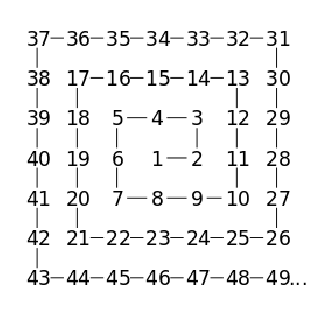
\includegraphics{spiral5.eps}
   
\item
  Дана матриця розміру $n \times m$. Поміняти місцями стовпці, що містять
  мінімальний і максимальний елементи матриці.
\item
  Дано дві матриці $n \times m$ і $m \times k$. Отримайте їх добуток.
\item
  Дана матриця розміру $n \times m$. Поміняти місцями її рядки так, щоб їх
  максимальні елементи утворювали зростаючу послідовність.
\item
  У даній дійсної квадратної матриці порядку $n$ знайти найбільший по
  модулю елемент.
\item
  Отримати квадратну матрицю порядку $n - 1$ шляхом викидання з вихідної
  матриці будь-якого рядка і стовпця, на перетині яких розташований
  елемент зі знайденим значенням. Виконуйте до тих пір, поки не
  залишиться останній елемент.
\item
  Дана квадратна матриця порядку $2n + 1$. Дзеркально відобразити її
  елементи відносно побічної діагоналі матриці.
\item
  Дана дійсна квадратна матриця порядку $2n + 1$. Отримати нову матрицю,
  повернувши її блоки, обмежені діагоналями, на 90 градусів.
\item
  Дана матриця розміру $n \times m$. Поміняти місцями її перший і останній
  рядки, що містять тільки негативні елементи.
\item
  Дана цілочисельна матриця розміру $n \times m$. Знайти елемент, який є
  максимальним у своєму рядку і мінімальним в своєму стовпці. Якщо такий
  елемент відсутній, то вивести 0.
\item
  Складіть програму циклічної перестановки стовпців двовимірного масиву
  $n \times m$, при якій зсуві зсувається вправо на $k$ стовпців.
\item
  Дана матриця розміру $n \times m$. Поміняти місцями її стовпці так, щоб їх
  мінімальні елементи утворювали зростаючу послідовність.
\item
  Дана квадратна матриця порядку $2n + 1$. Дзеркально відобразити її
  елементи відносно вертикальної оC симетрії матриці.
\item
  Дана квадратна матриця порядку $2n$. Повернути її на 270 градусів в
  додатньому напрямку щодо її центру.
\item
  Дана матриця розміру $n \times m$. Поміняти місцями рядки, що містять
  мінімальний і максимальний елементи матриці.
\item
  У квадратній таблиці обміняйте місцями елементи рядка і стовпця, на
  перетині яких знаходиться мінімальний з позитивних елементів.
\item
  Дана квадратна матриця порядку $2n$. Повернути її на 90 градусів в
  за годинниковою стрілкою щодо її центру.
\item
  Дана квадратна матриця порядку $2n + 1$. Дзеркально відобразити її
  елементи відносно головної діагоналі матриці.
\item
  Складіть програму циклічної перестановки рядків двовимірного масиву $n \times m$,
  при якій зсув відбувається вниз на $k$ рядків.
\item
  Дана матриця розміру $n \times m$. Поміняти місцями її перший і останній
  стовпці, що містять тільки позитивні елементи.
\item
  Заповнити двовимірний квадратний масив цілими числами від 1 до 100 по
  спіралі, починаючи від центру і закручуючи за годинниковою стрілкою.
\item
  Заповніть квадратну матрицю $n \times n$ за принципом латинського квадрата: в
  кожному рядку і кожному стовпці використовуються лише числа від 1 до n
  що не повторюються між собою.
\item
  Дана матриця дійсних коефіцієнтів. Впорядкувати її рядки по неспаданню
  перших елементів, суми значень рядків, величині найменших елементів
  рядків.
\end{enumerate}

\section{Додаткові задачі:}

\begin{enumerate}
\def\labelenumi{\arabic{enumi})}
\setcounter{enumi}{32}
\item
  Дана матриця $n \times m$ з нулів та одиниць. Знайти найбільший за площиною
  прямокутник з одних одиниць. Зробіть цю задачу без вкладених 4-х
  циклів для $0<n,m<255$.
\end{enumerate}


\chapter{Динамічні масиви. Робота з вказівниками }
%

\section{Контрольні запитання:}
\begin{itemize}
\item
  Як можна створити лінійний динамічний масив та коректно завершити при
  цьому програму?
\item
  Що таке вказівники? Які операції визначені на вказівниках? Як
  проітеруватись по даному масиву за допомогою вказівника?
\item
  Як визначити динамічну матрицю за допомогою масиву вказівників та
  коректно її обробити?
\item
  Які функції та з якої бібліотеки використовуються на C для виділення
  памяті? В чому їх різниця? Що відбудеться якщо потрібної пам'яті не
  було ними виділено?
\item
  Які функції існують для очищення пам'яті? Що відбудеться, якщо їх не
  використовувати? Які ще проблеми виникають при некоректному очищенні
  чи його відсутності?
\end{itemize}

\section{Завдання для аудіторної роботи:}

\begin{enumerate}
\def\labelenumi{\arabic{enumi})}
\item
  Ввести натуральне число $n$. Створити та ввести масив з $n$ дійсних чисел та
  підрахувати суму квадратів елементів цього масиву. 

\item
  Написати функцію, що вводить масив цілих чисел доки не введеться нуль
  через змінний аргумент та кількість елементів масиву повертається як
  результат роботи функції. Кількість елементів обмежена числом 100.
  Підрахувати кількість повних квадратів та кубів в цьому масиві.
\item
  Створити функцію, що вводить $n$-вимірний вектор ($n$
  задається як аргумент функції, результат -- вказівник на результатний масив),
 виділяючи відповідну пам'ять та функцію, що відповідно очищує пам'ять. 
 Напишіть програму, що вводить два вектори, підраховує та створює як окремий масив їх
  різницю якщо це можливо, та в будь-якому варіанті коректно
  завершує програму без витоків пам'яті.
\item
  Створити функції, що коректно ініціалізують нулями та вводять з консолі 
дійсну квадратну $n$-вимірну матрицю ($n$ задається як аргумент функції), й
  функцію, що відповідно очищує пам'ять. Напишіть програму, що вводить
  дві матриці, підраховує та обчислює як окремий масив їх добуток, якщо
  це можливо, та в будь-якому варіанті коректно завершує програму без
  витоків пам'яті. Зробіть дану задачу:
  \begin{itemize}
  \item
представляючі матрицю у вигляді двовимірного масиву;
  \item
представляючі матрицю у вигляді лінійного масиву розміру $n^{2}$.
 \end{itemize}

\end{enumerate}

\section{Завдання для самостійної роботи:}

\begin{enumerate}
\def\labelenumi{\arabic{enumi})}
\setcounter{enumi}{4}
\item
  Створити функцію, що вводить матрицю цілих чисел довільних
  розмірностей, виділяючи відповідну пам'ять (розміри масивів) та
  функцію, що відповідно очищує пам'ять. Напишіть функцію, що підраховує
  ранг матриці. Коректно протестуйте роботу цих функцій.
\item
  Створити функцію, що вводить матриці довільних розмірностей, виділяючи
  відповідну пам'ять та функцію, що відповідно очищує пам'ять. Напишіть
  програму, що вводить масив таких матриць, підраховує та створює як
  окремий масив добуток всього масиву матриць, якщо це можливо, та в
  будь-якому варіанті коректно завершує програму без витоків пам'яті.

\item
  Ввести натуральне число $n$. Створити та ввести масив з $n$ натуральних
 довгих чисел та підрахувати кількість ступенів двійки та трійки в цьому масиві.
\item
  Вирішіть завдання виконуючи наступні вимоги:

Сформувати динамічний двовимірний дійсний масив $N \times M$, заповнити його випадковими
числами або з консолі та вивести на екран. Виконати наступні дії, коректно оброблюючи 
всі можливі сценарії:

\begin{enumerate}[label=\xslalph*)]
\item
  додати рядок після заданого номеру $k$;
\item
  додати стовпець після заданого номеру $k$;
\item
  додати рядок в кінець матриці;
\item
  додати стовпець в кінець матриці;
\item
  додати рядок в початок матриці;
\item
  додати стовпець в початок матриці;
\item
  додати $k$ рядків в кінець матриці;
\item
  додати $k$ стовпців в кінець матриці;
\item
  додати $k$ рядків в початок матриці;
\item
  додати $k$ стовпців в початок матриці;
\item
  видалити рядок з номером $k$;
\item
  видалити стовпець з номером $k$;
\item
  видалити рядки, починаючи з рядка $k1$ і до рядка $k2$;
\item
  видалити стовпці, починаючи з стовпця $k$ і до стовпчика $k$;
\item
  видалити всі непарні рядки;
\item
  видалити всі парні стовпці;
\item
  видалити всі рядки, в яких є хоча б один нульовий елемент;
\item
  видалити всі стовпці, в яких всі елементи менші за 1;
\item
  видалити рядок, в якій знаходиться наймеший за модулем елемент матриці (
якщо їх декілька -- видалити усі);
\item
  додати рядок після кожного парного рядку матриці;
\item
  додати стовпець після кожного парного стовпця матриці;
\item
  додати $k$ рядків, починаючи з рядку за номером $m$;
\item
  додати $k$ стовпців, починаючи зі стовпчика за номером $m$;
\item
  додати рядок після рядка, що містить найбільший елемент;
\item
  додати стовпець після стовпця, що має найбільшу суму елементів;
\item
  додати рядок після рядка, що має найменше значення норми (суми квадратів)(
якщо їх декілька -- обираємо останній);
\item
  додати стовпець після стовпця, що містить найменший за модулем елемент (
якщо їх декілька -- обираємо перший);
\item
  видалити рядок і стовпець, на перетині яких знаходиться найбільший
  елемент матриці.
\end{enumerate}

\end{enumerate}

\section{Додаткові задачі:}

\begin{enumerate}
\def\labelenumi{\arabic{enumi})}
\setcounter{enumi}{8}
\item
  Користувачу надається можливість декілька разів вводити розмірність
  вектору дійсних чисел та самі ці значення. Після кожного вводу
  потрібно підрахувати середнє арифметичне та дисперCю всіх введених
  значень.
\item
  Петя та Вася кожен день на протязі $N$ днів вимірюють
  декілька (від 0 до 1000) разів температуру повітря (хоча інколи хтось
  може забути це зробити). Створіть програму, що дозволить їм ввести ці
  результати за кожен день спостережень та підрахує середню температуру
  кожного з цих днів, де сумарна кількість вимірювань була більше 1.
  Програма повинна передбачити, що після вводу цих $N$ днів вони можуть
  захотіти ввести наступні $M$ днів таких спостережень. Передбачте
  можливість коректного завершення при нестачі ресурCв комп'ютера для
  зберігання та обробки даних.
\item
 В масиві натуральних чисел A{[}N{]} всі числа є меншими 16. Напишить
  функцію, що зберігає дані цього масиву у масиві $N/2$ чисел типу
  uint8\_t (тобто в кожному числі uint8\_t зберігається два числа масиву
  A{[}i{]}).
\item
  В масиві натуральних чисел A{[}N{]} всі числа є меншими 64. Напишить
  функцію, що зберігає дані цього масиву у масиві $[N*4/3]$ чисел типу
  uint8\_t (тобто в кожних трьох числах uint8\_t зберігається чотири
  числа масиву A{[}i{]}).
\item
  В масиві натуральних чисел A{[}N{]} всі числа є меншими \(2^{k}\).
  Знайдіть це число $k$ та напишить функцію, що зберігає цей масив в $N*k$
  біт найбільш економічним чином( int A{[}3{]}, k=5 → uint8 B{[}2{]}
  ,тобто використовує 16 біт, або int A{[}8{]}, k=14 → uint16 B{[}7{]} ,
  тобто використовує 112 біт) та функцію що обратно повертає числа з
  масиву B у масив A.
\end{enumerate}



\chapter{Структури. Створення власного типу}
%

\section{Контрольні запитання:}
\begin{itemize}
\item Що таке структура та як її створити на C?
\item Як створити власний тип даних на C?
\item Як визначити структуру, що має посилання на саму себе?
\item Які варіанти ініціалізації структур? Як ввести структуру? Як отримати
структуру як результат роботи функції? Через змінний аргумент?
\item Нащо використовувати typedef при створенні власної структури?
\end{itemize}

\section{Завдання для аудиторної роботи:}

\begin{enumerate}
\def\labelenumi{\arabic{enumi})}
\item
  Визначити типи структури для зображення наступних понять та функції їх вводу-виводу:
 \begin{enumerate}[label=\xslalph*)]
 \item дата (число, місяць, рік);
 \item поле шахової дошки (напр., а5, b8);
 \item прямокутник зі сторонами, паралельними осям координат, заданий через дві вершини.
Вершина в свою чергу -- теж структура яка містить дві дійсні координати;
 \item поліном довільного ступеня (ступінь поліному та дійсні коефіцієнти --- безрозмірний
масив).
 \end{enumerate}

\item
 Використовуючи тип Поле шахової дошки описати булеву функцію, яка
перевіряє, чи може за один хід ферзь перейти з одного заданого поля
шахової дошки на інше задане поле.

\item
 Використовуючи опис типу Дата, визначити функції обчислення:
дати завтрашнього дня та дня тижня за його датою в поточному році.

\item
 Визначимо тип Rational (Раціональне число) як:
\begin{verbatim}
typedef struct {
int numerator; // чисельник
unsigned int denominator; // знаменник
} Rational;
\end{verbatim}

Визначити функції для:
\begin{itemize}
\item обчислення суми двох раціональних чисел;
\item обчислення добутку двох раціональних чисел;
\item порівняння двох раціональних чисел;
\item зведення раціонального числа до нескоротного виду.
\end{itemize}


\item
 Задано масив розмірності N, компонентами якого є структури, що містять відомості про вершини гір. У
відомостях про кожну вершину вказуються назва гори та її висота.
Визначити функції введення/виведення гір та функції пошуку назви
найвищої вершини та виведення висоти вершини з заданою назвою (якщо
вершини з такою назвою немає в масиви -- вивести відповідне
повідомлення).
\end{enumerate}

\section{Завдання для самостійної роботи:}

\begin{enumerate}
\def\labelenumi{\arabic{enumi})}
\setcounter{enumi}{5}
\item
 Визначити типи запису для зображення наступних понять та реалізуйте
їх функції введення виведення:
\begin{enumerate}[label=\xslalph*)]
\item ціна (гривні, копійки);
\item час (година, хвилина, секунда);
\item повна дата (число, місяць, рік, година, хвилина);
\item адреса (місто, вулиця, будинок, квартира);
\item семінар (предмет, викладач, № групи, день тижня, години занять, аудиторія);
\item бланк вимоги на книгу (відомості про книгу: шифр, автор, назва;
відомості про читача: № читацького квитка, прізвище; дата замовлення);
\item коло (радіус, координати центра);
\item сфера в просторі;
\item прямокутний паралеліпипед (сторони якого паралельні вісям координат);
\item вектор (розмір вектору -- натуральне число та масив дійсних значень);
\item матриця (розміри матриці -- два натуральних числа та масив дійсних значень);
\item багатокутник (розмір багатокутнику та набір координат вершин).


\end{enumerate}

\item
  В масиві структур записано вартість та вік кожної з N моделей легкових
  автомобілів. Визначити середню вартість автомобілів, вік яких більший
  за 5 років.
\item
  В масиві структур записано інформацію про ціну та наклад кожного з N
  журналів. Знайти середню вартість журналів, наклад яких менший за
  10000 примірників.
\item
  В масиві структур записано дані про масу й об'єм N предметів,
  виготовлених із різних матеріалів. Знайти предмет, густина матеріалу
  якого найбільша.
\item
  В масиві структур записано дані про чисельність населення (у мільйонах
  жителів) та площі N держав. Знайти країну з мінімальною щільністю
  населення.
\item
  Задано масив P розмірності N, компонентами якого є відомості про
  мешканців деяких міст. Інформація про кожного мешканця містить його
  прізвище, назву міста, місцеву адресу у вигляді вулиці, будинку,
  квартири. Визначити функцію пошуку двох будь-яких жителів, що мешкають
  у різних містах за однаковою адресою.
\item
  Відомо дані про вартість кожного з N найменувань товарів: кількість
  гривень, кількість копійок. Скласти підпрограми пошуку:
\begin{enumerate}[label=\xslalph*)]
\item найдешевшого товару в магазині;
\item найдорожчого товару в магазині;
\item товару, вартість якого відрізняється від середньої вартості 
товару в магазині не більш ніж на 10 гривень:

\end{enumerate}

\item
  Задано масив Р розмірності N, компонентами якого є стурктури, що
  містять анкети службовців деякого закладу. У кожній анкеті вказуться
  прізвище та ім'я службовця, його стать, дата народження у вигляі
  числа, місяця, року. Визначити підпрограми пошуку:
\begin{enumerate}[label=\xslalph*)]
\item посади, яку обіймає найбільша кількість співробітників;
\item співробітників з однаковими іменами;
\item співробітників, прізвища яких починаються із заданої літери;
\item найстаршого з чоловіків цього закладу;
\item співробітників, вік яких менший за середній по організації;
\item пенсійного віку (урахувати, що пенсійний вік чоловіків і жінок --
різний).
\end{enumerate}

\item
  Задано масив $P$, компонентами $P_i$ якого є записи, що містять дані про
  людину на ім'я $i$ з указаного списку. Кожне дане складається зі статі
  людини та її зросту. Визначити підпрограми для:
\begin{enumerate}[label=\xslalph*)]
\item обчислення середнього зросту жінок;
\item пошуку найвищого чоловіка;
\item перевірки, чи є дві людини, однакові на зріст.
\end{enumerate}

\item
  Задано масив розмірності N, компоненти якого містять інформацію про
  студентів деякого вишу. Відомості про кожного студента містять дані
  про його прізвище, ім'я, по батькові, стать, вік, курс. Визначити
  процедуру пошуку:
\begin{enumerate}[label=\xslalph*)]
\item найпоширеніших чоловічих і жіночих імен;
\item прізвищ та ініціалів усіх студентів, вік яких є найпоширенішим.
\end{enumerate}

\item
  Задано масив розмірності N, компонентами якого є відомості про
  складання іспитів студентами деякого вишу. Інформація про кожного
  студента задана в такому вигляді: прізвище, номер групи, оцінка\_1,
  оцінка\_2, оцінка\_3. Визначити процедуру пошуку:
\begin{enumerate}[label=\xslalph*)]
\item студентів, що мають заборгованості принаймні з одного з предметів;
\item предмета, складеного найгірше;
\item студентів, що склали всі іспити більше заданої оцінки.
\end{enumerate}

\end{enumerate}

\section{Додаткові задачі:}

\begin{enumerate}
\def\labelenumi{\arabic{enumi})}
\setcounter{enumi}{17}
\item
  Визначити універсальний тип, який допускає зображення точки на площині
  у прямокутній або полярній системі координат (3-тє поле -- тип
  координат). Побудувати функцію обчислення площі трикутника з вершинами
  A, B, C.
\end{enumerate}


\chapter{Робота з бінарними файлами на C}
%

\section{Контрольні запитання:}
\begin{itemize}
\item
  Цикл роботи з файлами на C/C++.
\item
  Як створити та працювати з текстовим файлом на C? Як можна вводити та
  виводити файл посимвольно? Порядково?
\item
  Чим відрізняється бінарний файл від текстового? 
\item 
  Як створити бінарний файл? Як читати з бінарного файлу?
\item
  Як записати та прочитати масив дійсних чисел в/з бінарного файлу?
\item
  Як прочитати всі цілі числа з файлу, якщо на початку роботи невідомо,
  скільки їх там насправді?
\item
  Які додаткові речі можна робити з бінарним файлом, що неможна робити з
  текстовим?
\item
  Як записати масив структур у файл та прочитати k-тий запис у файлі?
\end{itemize}

\section{Завдання для аудиторної роботи:}

\begin{enumerate}
\def\labelenumi{\arabic{enumi})}

\item
Введіть довжину масиву дійсних чисел та сам масив. Реалізуйте функцію, яка 
запише цей масив в файл з заданим ім'ям. Реалізуйте функцію, що виведе вміст 
файлу з дійсних чисел на консоль в одному рядку через коми. 


\item
  Використовуючи файл F, компоненти якого є дійсними числами, побудувати
  файл G, що містить усі числа з файлу F, які менші по модулю за задане число $a>0$.
  Послідовність чисел зберігається. Після цього видалити всі елементи з файлу F, 
  які менші по модулю за число $a$.

\item
  Створіть файл F, компоненти якого є цілими числами. При цьому введення
цілих чисел робиться в нескінченому циклі, доки користувач не введе 0. 
 Побудувати файл G, який містив би всі компоненти файлу F:
\begin{enumerate}[label=\xslalph*)]
\item
що є парними числами; 
\item
 що діляться на 3 і на 5;
\item
що є точними квадратами; 
\item
що мають лише 3 дільники; 
\item
що є паліндромами;
\item
що є числами Фібоначчі.
\end{enumerate}


\item
  Створить файл, який містить відомості про прямокутники: вказано номер
  прямокутника у файлі, координати (дійсні числа) верхнього лівого кута та
  нижнього правого кута прямокутника. Скласти функцію пошуку
  прямокутника з найбільшою площею й визначення цієї площі.
\item
  У файлі компоненти -- структури вигляду $(coef, deg, num )$ -- 
дійсний коефіцієнт, ступінь члену полінома ($koef \ge 0$) та номер поліному. 
Таким чином в файлі записано декілька поліномів (номер поліному встановлює
до якого поліному належить цей член).
Визначити підпрограми для
  виконання наступних дій над поліномом:

\begin{enumerate}[label=\xslalph*)]
\item
введення полінома та запис (додавання) його в файл; 
\item
друк полінома з файлу за номером на консоль у звичному вигляді поліному від $x$;
\item
обчислення похідної від полінома за файлом та номером;
\item
додавання поліному у файл заданий іменем;
\item
видалення поліному за даним номером;
\item
заміна коефіцієнту заданого ступенем та номером поліному;
\item
заміна коефіцієнту заданого номером структури(компоненти) у файлі.
\end{enumerate}

\end{enumerate}


\section{Завдання для самостійної роботи:}

\begin{enumerate}
\def\labelenumi{\arabic{enumi})}
\setcounter{enumi}{4}
\item
  Дано файл, компоненти якого є натуральними числами. Скласти
  підпрограми для обчислення:
\begin{enumerate}[label=\xslalph*)]
\item
кількості парних чисел серед компонент;
\item
кількості квадратів непарних чисел серед компонент;
\item
різниці між найбільшим парним і найменшим непарним числами компонент;
\item
кількості простих чисел серед компонент;
\item  
кількості компонент у найдовшій зростаючій послідовності компонент
файлу.
\end{enumerate}

\item
  Дано файл, компоненти якого є дійсними числами. Скласти підпрограми
  для обчислення:
\begin{enumerate}[label=\xslalph*)]
\item
суми компонент файлу;
\item
кількості від'ємних компонент файлу;
\item
останньої компоненти файлу;
\item
передостанньої компоненти;
\item 
найбільшої по модулю компоненти файлу;
\item
найменшої з компонент файлу з парними номерами;
\item 
суми найбільшої та найменшої з компонент;
\item
різниці першої й останньої компоненти файлу;
\item
кількості компонент файлу, які менші за середнє арифметичне всіх його
компонент.
\end{enumerate}


\item
  Задано натуральне число $n$ та файл F, компоненти якого є цілими
  числами. Побудувати файл G, записавши до нього найбільше значення
  перших $n$ компонент файлу F, потім -- наступних $n$ компонент тощо.
  Розглянути два випадки:
\begin{itemize}
\item
кількість компонент файлу ділиться на $n$;
\item
кількість компонент файлу не ділиться на $n$. 
\end{itemize}
Остання компонента файлу G має дорівнювати найбільшій із компонент 
файлу F, які утворюють останню (неповну) групу.

\item
  Дано файл F, компоненти якого є цілими числами. Файл містить рівну
кільксть додатних і від'ємних чисел -- перевірте це і в противному
  випадку видайтие відповідне повідомлення та не робить нічого.
  Використовуючи допоміжний файл H, переписати компоненти файлу F до
  файлу G так, щоб у файлі G:
\begin{enumerate}[label=\xslalph*)]
\item
не було двох сусідніх чисел одного знаку;
\item
спочатку йшли додатні, потім -- від'ємні числа;
\item
числа йшли таким чином: два додатних, два від'ємних тощо. Якщо це
неможливо -- то переписати поки можливо в такому вигляді, а останні два
числа вивести на консоль.
\end{enumerate}

\item
  Дано файл F, компонентами якого є записи (структури) вигляду
\begin{verbatim}
struct T {
unsigned Key; // ключ
char Data[10]; // дані
};
\end{verbatim}

Такий файл називатимемо впорядкованим за ключами, якщо записи в ньому
розташовуються в порядку зростання (спадання) ключів. Скласти процедуру
пошуку запису за ключем у впорядкованому файлі. Скласти процедуру
вилучення запису із заданим ключем:
\begin{itemize}
\item з впорядкованого файлу;
\item з невпорядкованого файлу.
\end{itemize}

\item
  Багаж пасажира характеризується номером пасажира, кількістю речей і
  їхньою загальною вагою. Дано файл пасажирів, який містить прізвища
  пасажирів, і файл, що містить інформацію про багаж декілька пасажирів
  (номер пасажира -- це номер запису у файлі пасажирів). 
Скласти процедури для:
  \begin{enumerate}[label=\xslalph*)]
\item
знаходження пасажира, у багажі якого середня вага однієї речі
відрізняється не більш ніж на 1 кг від загальної середньої ваги речей;
\item
визначення пасажирів, які мають більше двох речей, і пасажирів
кількість речей у яких більша за середню кількість речей;
\item
видачі відомостей про пасажира, кількість речей у багажі якого не
менша, ніж у будь-якому іншому багажі, а вага речей -- не більша, ніж у
будь-якому іншому багажі із цією самою кількістю речей;
\item
визначення, чи мають принаймні два пасажири багажі, які не
відрізняються за кількістю речей і відрізняються вагою не більш ніж на 1
кг (якщо такі пасажири є, то показати їхні прізвища);
\item визначення пасажира, багаж якого складається з однієї речі вагою не
менше $m$ кг.
  \end{enumerate}

\item
  Дано файл, який містить відомості про іграшки: указано назву іграшки
  (напр., м'яч, лялька, конструктор тощо), її вартість у гривнях і
  вікові межі для дітей, яким іграшка призначається (напр., для дітей
  від двох до п'яти років). Скласти функції, що виводять наступні результати 
  у бінарний файл та на консоль:

  \begin{enumerate}[label=\xslalph*)]
\item
пошуку назв іграшок, вартість яких не перевищує заданої кількості гривень,
 призначених дітям п'яти років;
\item
пошуку назв іграшок, призначені дітям і чотирьох, і десяти років;
\item
пошуку назв найдорожчих іграшок (ціна яких відрізняється від ціни
найдорожчої іграшки не більш ніж на 50 грн);
\item визначення ціни найдорожчого конструктора;
\item визначення ціни всіх кубиків;
\item пошуку двох іграшок, що призначені дітям трьох років, сумарна
вартість яких не перевищує X грн;
\item
пошуку конструктора ціною Y грн, призначеного дітям від п'яти до
десяти років. Якщо такої іграшки немає, то занести відомості про її
відсутність до файлу.
  \end{enumerate} 


\end{enumerate}

\section{Додаткові задачі:}

\begin{enumerate}
\def\labelenumi{\arabic{enumi})}
\setcounter{enumi}{11}
\item
  У двох файлах міститься таблиця футбольного турніру, у першому --
  записано назви команд; у другому -- результати матчів, що зберігаються
  у записах типу T\_Match:
\begin{verbatim}
typedef struct {
unsigned int n1, n2;
unsigned int b1, b2;
} T_Match;
\end{verbatim}
Тут у структурі типу T\_Match поля n1, n2 -- номери першої і другої 
команд (тобто номери назв команд у файлі команд); b1, b2 -- кількість
м'ячів, забитих першою та другою командами, відповідно.
Кожній команді за перемогу нараховується 3 очки, за нічию -- 1, за
поразку -- 0.
Із двох команд, які мають однакову кількість очок, першою вважається:
\begin{itemize}
\item
та, що має кращу різницю забитих і пропущених м'ячів;
\item
за однакової різниці має більше забитих м'ячів;
\item
за всіма однаковими попередніми показниками визначається жеребкуванням
(для жеребкування використати генератор випадкових чисел).
\end{itemize}
Знайти команду, яка є лідером.

\emph{Вказівка.} Описати підпрограми створення файлів команд і матчів, 
додавання результату матчу, визначення лідера.

\item
Файл бази даних з малюнками містить на початку ціле 32-бітне число
2051, потім ціле 32-бітне число $K$ --- кількість малюнків, а наступні два
32-бітних числа $n,m$ --- висота та ширина кожного малюнку у
пікселах. При цьому ці числа задані в форматі big-indian.
Наступний вміст файлу -- беззнакові натуральні байти ($K*n*m$ байтів),
кожен з яких -- значення яскравостей пікселів (число від 0 до 255)
кожного з цих малюнків, що проходяться у порядку зліва-направо та
згору-донизу.

Напишіть функцію, що перевіряє даний файл (заданий ім'ям) на
відповідність даному формату та виводить масив яскравостей малюнка з
заданим номером, якщо такий номер та сам файл коректно задані. В
противному випадку вивести змістовне повідомлення про помилку.

\end{enumerate}


\chapter{Введення/виведення на С++. Робота з текстовими файлами на C++}
%

\section{Контрольні запитання:}
\begin{itemize}

\item
  Як використовувати бібліотеки C на C++? Що потрібно для того щоб код
  на C працював так само на C++?
\item
  Яка різниця булевого типу та його використання на C та C++?
\item
  Як вивести в C++ використовуючи потоки виведення дійсне число з
  заданою точністю? В науковому представленні? З заданою шириною?
\item
  Як записати у текстовий файл масив цілих чисел через кому у якості
  роздільника та прочитати потім цей масив?
\item
  Що таке перевантаження функцій та навіщо воно може бути потрібно?
\item
  Що таке new та new{[}{]}? Коли потрібно перше та коли друге?
\item
  В чому різниця між new та malloc?
\item
  Як очищувати пам'ять після new та new{[}{]}?
\end{itemize}

\section{Завдання для аудиторної роботи:}

\begin{enumerate}
\def\labelenumi{\arabic{enumi})}
\item
  Ввести в двох різних рядках послідовно два дійсних числа $x$ та $y$ та
  обчислити значення $x$ в ступені $y$. Результат вивести в десятковому та
  науковому представленні.
\item
  На терміналі вводяться $10*n$ цифр. Перші 10 цифр -- це перше натуральне
  число, наступні 10 -- друге і так далі. Введіть всі ці числа в масив
  розміру $n$ та обчисліть і виведіть їх суму (вважайте що сума влазить в
  точність unsigned long long).
\item
  Вивести на екран таблицю для всіх чисел від 1 до $n$ 
 (організувати прицьому переноси на нові рядки для заданої довжини), 
  слідкуючи, щоб виведення було рівним та кількість цифр після коми була або 0 або 2:
\begin{verbatim}
++++++++++++++++++++++++++++++++++++++++
   1       2       3       4       5 
++++++++++++++++++++++++++++++++++++++++
   1    1.41    1.73       2    2.24 
++++++++++++++++++++++++++++++++++++++++
\end{verbatim}
\item
  Ввести з текстового файлу та з консолі натуральне число $n$ та масиви з
  $n$ цілих чисел \(\left\{ m_{i} \right\}_{i = 1}^{n}\) та дійсних чисел
  \(\left\{ x_{i} \right\}_{i = 1}^{n}\). Обчислить та виведіть у файл
  числа \(\left\{ x_{i}^{m_{i}} \right\}_{i = 1}^{n}\).
\item
  Вхідний потік заданий текстовим файлом містить набір цілих чисел $A_i (0
  \le A_i \le 10^{18}$), відділений один від іншого довільною кількістю пробілів
  і переводів рядків. Розмір вхідного потоку не перевищує 256 КБ. Для
  кожного числа $A_i$, починаючи з останнього та завершуючи першим, в
  окремому рядку вивести його квадратний корінь не менш ніж з чотирма
  знаками після десяткової крапки.

Приклад:

\textbf{Вхід:}
\begin{verbatim}
1427      0

   876652098643267843

5276538
\end{verbatim}
\textbf{Вихід: }

2297.0716

936297014.1164

0.0000

37.7757

\end{enumerate}

\section{Завдання для самостійної роботи:}

\begin{enumerate}
\def\labelenumi{\arabic{enumi})}
\setcounter{enumi}{5}
\item
  Ввести декілька (невідомо зазделегідь скільки) дійсних числа записаних
  через коми та обчислити значення функції $log()$ для кожного з них. Якщо
  значення виходить за межі області вивести слово ``None'', для інших
  значень результат вивести в науковому та десятковому представленні
  шириною 5 символів.
\item
  Три додатних дійсних числа вводяться як рядок вигляду \\
  А=ххх.ххх, B=xxExxx C=xxx.xxxx\\
  Обчисліть їх середнє гармонічне та виведіть у науковому та звичайному
  форматі.
\item
  Ввести дійсне число від -10000 до 10000 та вивести його $k$-ту ступінь
  ($|k|<10$) з точністю до 20 знаків до десяткової коми та 4
  знаками після десяткової коми (нуль залишається нулем завжди).
\end{enumerate}

\textbf{Даний блок задач вимагає організувати роботу з текстовим файлом.
 Вихідні файли не передбачають зміни. Змінені дані зберігаються в іншому файлі.}

\begin{enumerate}
\def\labelenumi{\arabic{enumi})}
\setcounter{enumi}{8}
\item
  Дано два текстові файли з іменами Name1 і Name2. Додати в кінець
  кожного рядка файлу Name1 відповідний рядок файлу Name2. Якщо файл
  Name2 коротший файлу Name1, то виконайте перехід до початку файлу
  Name2.
\item
  Організувати текстовий файл, що складається з N рядків. Визначити
  максимальний і мінімальний розмір рядків в файлі і вивести їх в інший
  файл.

\item
  Дано символ $c$ (прописна латинська літера) і текстовий файл. Створити
  текстовий файл, який містить всі слова з вихідного файлу, що
  починаються цією літерою (як великої, так і малої). Розділові знаки,
  розташовані на початках і в кінцях слів, не враховувати. Якщо вихідний
  файл не містить відповідних слів, залишити результуючий файл порожнім.
\end{enumerate}

\textbf{Даний блок задач вимагає організувати роботу з текстовим файлом. 
Вхідний файл потрібно змінити згідно вказаних умов, тобто вхідний та вихідні файли
співпадають.}

\begin{enumerate}
\def\labelenumi{\arabic{enumi})}
\setcounter{enumi}{12}
\item
  Дано число N і текстовий файл. Видалити з файлу рядки з номерами,
  кратними N. Порожні рядки не враховувати і не видаляти. Якщо рядки з
  необхідними номерами відсутня, то залишити файл без змін. Зміна
  вивести в другий файл.
\item
  Дан текстовий файл, що містить текст, вирівняний по лівому краю
  (довжина кожного рядка не перевищує 50 символів). Вирівняти його по
  центру, додавши в початок кожної непорожній рядки необхідну кількість
  прогалин. Рядки непарної довжини перед центруванням доповнювати зліва
  прогалиною. Вирівняний текст записати в інший файл.
\item
  Організувати текстовий файл, що складається з N рядків. Перетворити
  файл, видаливши в кожній його рядку зайві пробіли. Зміни вивести в
  другий файл.
\item
  Дан файл з текстом із символів латинського алфавіту. Зашифрувати файл,
  виконавши циклічний зсув кожної букви вперед на n позицій в алфавіті.
  Розділові знаки і пропуски не змінювати.
\item
  Дано числа N1, N2 і текстовий файл. Видалити з файлу рядки з номерами
  між N1, N2, не включаючи меж. Зміни вивести в другий файл. Якщо
  виконати видалення неможливо, видайте про це повідомлення на екран і в
  вихідний файл.
\item
  Даний файл з текстом із символів латинського алфавіту, цифр та знаків.
  Замініть всі цифри їх назвами на англійській мові.
\item
  Створити текстовий файл F, що складається з N рядків. Після цього
  створити файли H і G. У файл H записати рядки файлу F непарної
  довжини, в файл G парної довжини.

\item
 Визначити функцію, яка:
\begin{itemize}
\item підраховує кількість порожніх рядків;
\item обчислює максимальну довжину рядків текстового файлу.
\end{itemize}

\item Визначити процедуру виведення:
\begin{itemize}
\item усіх рядків текстового файлу;
\item рядків, які містять більше 60 символів.
\end{itemize}

\item
Визначити функцію, що визначає кількість рядків текстового файлу,
які:
\begin{itemize}
\item починаються із заданого символу;
\item закінчуються заданим символом;
\item починаються й закінчуються одним і тим самим символом;
\item що складаються з однакових символів.
\end{itemize}

\item
В даному текстовому файлі знаходиться англомовний текст. Вирівняйте
його по лівий та правий границі так щоб розподіл слів у рядках був
найбільш рівномірним.

\item
Визначити процедуру, яка переписує до текстового файлу G усі 
рядки текстового файлу F:
\begin{itemize}
\item із заміною в них символу '0' на '1', і навпаки;
\item в інвертованому вигляді.
\end{itemize}

\item
Визначити процедуру пошуку найдовшого рядка в текстовому файлі.
Якщо таких рядків кілька, знайти перший із них.
\item
Визначити процедуру, яка переписує компоненти текстового 
файлу F до файлу G, вставляючи до початку кожного рядка один символ пропуску.
Порядок компонент не має змінюватися.
\item
У текстовому файлі записано непорожню послідовність дійсних чисел,
які розділяються пропусками. Визначити функцію обчислення найбільшого з
цих чисел.

\item
У текстовому файлі F записано послідовність цілих чисел, які розділяються пропусками. 
Визначити процедуру запису до текстового файлу G усіх додатних чисел із F.

\item
У текстовому файлі кожний рядок містить кілька натуральних чисел, які розділяються пропусками.
Числа визначають вигляд геометричної фігури (номер) та її розміри. Прийнято такі домовленості:
\begin{itemize}
\item
відрізок прямої задається координатами своїх кінців і має номер 1;
\item
прямокутник задається координатами верхнього лівого й нижнього правого кутів і має номер 2;
\item
коло задається координатами центра й радіусом і має номер 3.
\end{itemize}

Визначити процедури обчислення:
\begin{itemize}
\item відрізка з найбільшою довжиною;
\item прямокутника з найбільшим периметром;
\item кола з найменшою площею.
\end{itemize}


\item 
У файлі записані координати точок на площині задані парою цілих
чисел. Точки записуються в форматі : ( х1 , х2 ) (х1 , х2) , \ldots{} --
саме так через коми та дужки. Створити файл, в якому будуть записані
координати всіх відрізків з точок цього файлу, при цьому ці відрізки
відсортовані за зростанням довжини.

\item 
У файлі записані координати Точок в просторі задані трійкою цілих
чисел. Точки записуються в форматі : х1 , х2 , х3 ; х1 , х2, х3;
\ldots{} Знайти відрізок з точок цього файлу, що має найбільшу довжину.

\item 
У файлі записані координати матеріальних точок на площині задані
парою цілих чисел та масою(дійсне число). Точки записуються в форматі :
{[}х1 , y1, m1 {]}, {[}х2 , y2, m2{]} , \ldots{}  -- саме так
через коми та дужки. Знайдіть дві точки з найбільшим важілем сили (m*(х
+y)).

\item 
У файлі записані дати , що задані трійкою цілих чисел у форматі
(чч1./мм1/рр1),(чч2./мм2/рр2), \ldots{} -- саме в такому форматі.
Створити файл, в якому будуть записано найстарша та найсвіжіша дати
(вважайте, що роки дат з 1951 по 2049).

\end{enumerate}

\section{Додаткові задачі:}
\begin{enumerate}
\def\labelenumi{\arabic{enumi})}
\setcounter{enumi}{33}

\item  Розглянемо послідовність чисел \(a_{i}\) , $i = 0, 1, 2, \ldots$, що
задовольняють умовам:

\(a_{0} = 0\), \(a_{1} = 1\); та \(a_{2i} = a_{i}\) і
\(a_{2i + 1} = {2a}_{i} + 1\) для кожного $i = 1, 2, 3, \ldots{} $.

Напишіть програму, яка для заданого значення $n$ знаходить максимальне
серед чисел \(a_{0},a_{1},\cdots,a_{n}\). Вхідні дані складаються з
декількох тестів (не більше 10). Кожен тест - рядок, в якому записано
ціле число $n$ ($1 \le n \le 99 999$). В останньому рядку вхідних даних записано
число 0. Для кожного $n$ у виводі запишіть максимальне значення.

\item
Створити текстовий (.txt) файл з 100,000,000 рядків з числами
в діапазоні від 0 до 999,999,999. Формат чисел - 9 знаків 
(1 = 000000001, 65535 = 000065535), всі числа розташовані в випадковому порядку без
повторів (кожен рядок -- унікальне число).

\emph{Приклад.}

000603453
 
914645283 

700500041 

035827127 
\end{enumerate}


\chapter{Робота з класом рядок на С++.}
%

\section{Контрольні запитання:}
\begin{itemize}
\item
  Які конструктори для класу рядок? Які для копі-конструкторів? Скільки та
  які оператори є перевантаженими для класу рядок?
\item
  Як видалити підрядок використовуючи методи класу String?
\item
  Як можна проітеруватись по рядку C++?
\item
  Як узнати довжину рядка?
\item
  Як знайти перше входження даного підрядку в рядку? Останнє?
\item
  Як вивести всі слова в реченні, що розділено пробілами? Комами?
\end{itemize}

\section{Завдання для аудиторної роботи:}

В даній групі задач потрібно реалізувати функції та в тих функціях де
потрібно виводити рядок зробіть 2 варіанти: 1) результат записати в
новий рядок; 2) результат замінює рядок, що є аргументом функції.

\begin{enumerate}
\def\labelenumi{\arabic{enumi})}
\item
  Даний рядок, що складається з символів латинського алфавіту,
  розділених пробілами (одним або декількома). Визначити кількість слів,
  які починаються і закінчуються однією і тією ж літерою.
\item
  Даний рядок, що складається з символів латинського алфавіту,
  розділених пробілами (одним або декількома). Перетворити кожне слово в
  рядку, видаливши з нього всі входження останньої літери цього самого
  слова (кількість пропусків між словами не змінювати).
\item
  Даний рядок із символів латинського алфавіту. Перевірте правильність
  розстановки тега \textless{}td\textgreater{}: кожному відкритого тегу
  повинен відповідати закритий \textless{}/ td\textgreater{}.
\item
  Даний рядок -- речення з символів латинського алфавіту. Вивести
  найкоротше слово в реченні. Якщо таких слів декілька, то: 
  а) вивести перше з них; б) останнє з них; в) всі такі слова.
\item
  У реченні, що складається зі слів, відокремлених одним пропуском,
  замінити першу букву у слів, що настають за словами die, der, das, на
  велику.
\item
  Напишіть функцію часткового спліттінгу рядку, тобто функцію, що
  приймає рядок та повертає перше слово з рядку (роздільник -- задається
  як аргумент функції)
\item
  Напишіть функцію, що приймає рядок та повертає масив (як
  аргумент-змінний) всі дійсні числа, що містяться в рядку (роздільник
  задається як аргумент функції)
\item
  У записці слова зашифровані -- кожне з них записано навпаки.
  Розшифрувати повідомлення. Слова розділяюьтся пробілами (довільною кількістю)
  та знаками коми, крапки, окличним та питання. 
\end{enumerate}

\section{Завдання для самостійної роботи:}

\begin{enumerate}
\def\labelenumi{\arabic{enumi})}
\setcounter{enumi}{8}
\item
  Даний рядок, що складається з символів латинського алфавіту,
  розділених пробілами (одним або декількома). Вивести рядок, що містить
  ці ж слова, але розділені одним символом ',' (кома). В кінці
  поставити крапку.
\item
  Даний рядок, що складається з символів латинського алфавіту,
  розділених пробілами (одним або декількома). Перетворити кожне слово в
  рядку, видаливши з нього всі входження останньої літери цього слова
  (кількість пропусків між словами не змінювати).
\item
  Речення складається з слів, розділених одним або декількома
  пропусками або комами. Написати програму, що друкує все слова, що закінчуються на
  заданий символ.
\item
  Даний рядок, що складається з символів латинського алфавіту,
  розділених пробілами (одним або декількома). Перетворити кожне слово в
  рядку видаливши з нього всі входження заданого символу (кількість
  пропусків між словами не змінювати).
\item
  Даний рядок-речення з символів латинського алфавіту. Перетворити рядок
  так, щоб кожне слово починалося з великої літери.
\item
  Даний рядок-речення з символів латинського алфавіту. Вивести найдовше
  слово в реченні (якщо таких слів кілька, то вивести останнє з них).
\item
  Визначити, скільки разів в рядку зустрічається задане слово.

\item
  Даний рядок, що складається з символів латинського алфавіту,
  розділених пробілами (одним або декількома). Визначити кількість слів,
  які містять введений символ.
\item
  Речення складається з слів, розділених одним або декількома
  пропусками. Написати програму, що друкує все слова, що закінчуються на
  введений символ.
\item
  У англійському реченні слова розділені одним пропуском. У всіх словах, що 
слідують за словами-артиклями a, an та the першу букву замінити на маленьку.
  Написати програму, що виконує цю роботу.
\item
  Написати програму, що визначає, який відсоток слів в англійському
  тексті містить подвоєну приголосну.
\item
  У мові використовується латинський алфавіт, причастя завжди
  закінчується суфіксом "ings". Заданий рядок слів, в якому слова
  відокремлюються одним або декількома пропусками. Надрукувати всі причастя
  з даного рядку.
\item
  Даний рядок з малих символів латинського алфавіту. Замініть кожен
  символ на наступний за ним за алфавітом, символ 'z' замініть на 'a'.
\item
  Даний рядок із символів латинського алфавіту. Замініть всі входження
  рядків ``one'', ''two'',''three``,\ldots{},''nine'' на символи `1',
  '2','3',\ldots{},'9'.
\item
  Відредагувати задане речення, видаляючи з нього ті слова, які
  зустрічаються в реченні задану кількість разів.
\item
  Визначте, який відсоток символи кожного слова складають з символів
  даного речення.
\item
  Даний текст, що складається з символів латинського алфавіту, пробілів і
  знаків пунктуації. Знайдіть найпоширенішу голосну букву (без
  урахування регістру).

\end{enumerate}

\section{Додаткові задачі:}

\begin{enumerate}
\def\labelenumi{\arabic{enumi})}
\setcounter{enumi}{27}
\item
  Даний рядок в якому зустрічаються слова, які складаються з восьми
  цифрових символів. Переведіть всі їх в формат дати "dd-mm-yyyy" і
  перевірте коректність такої дати.
\item
  В текстовому файлі записані в кожному рядку значення поліномів за
  допомогою знаків +, -, *, **(ступінь) та цифр і літери $x$. Введіть
  значення $x$ з консолі та для всіх коректних запиCв поліномів обчисліть
  їх значення для даного $x$ та виведіть в новий текстовий файл.
\end{enumerate}


\chapter{Створення власних класів. Інкапсуляція.}
%

\section{Контрольні запитання:}
\begin{itemize}
\item
Що таке класи і які шляхи визначення класів в C++?
\item
Яким чином можна визначити методи класу?
\item
Приватний та публічний доступ до членів та методів. Яка різниця?
\item
Які методи в класі визначені за замовченням? Як і коли потрібно ці
методи визначати самостійно?
\item 
Шляхи визначення конструктору класу. Як викликати конструктор в
головній функції?
\item
Статичні члени та методи класу. Як визначити і коли вони потрібні?
\item 
Дружні класи та методи. Як вони використовуються?
\end{itemize}

\section{Завдання для аудиторної роботи:}
\begin{enumerate}
\def\labelenumi{\arabic{enumi})}

\item 

Визначити клас раціональне число з членами: nominator --- ціле
число, denominator --- натуральне число. Визначить наступне:
\begin{itemize}
\item
методи введення та виведення з терміналу;
\item 
методи додавання та множення раціонального числа;
\item
зробіть члени класу приватними та визначить методи ініціалізації
окремо чисельника і знаменника (при цьому не дайте користувачу
можливість ініціалізувати знаменник нулем);
\item
cтворіть приватний метод класу для скорочення раціонального числа
через НСД;
\item визначить конструктори класу який ініціалізує за замовченням
раціональне число одиницями та конструктор, що ініціалізує його двома
довільними числами;
\item також у класі перевантажте основні арифметичні оператори, оператори
порівняння та інші оператори, що необхідні для роботи з раціональними
числами.
\end{itemize}

Використовуючи цей клас, розв'яжіть такі задачі:
\begin{itemize}
\item
знайдіть найменше раціональне число в масиві раціональних чисел;
\item
підрахуйте суму ряду за формулою Грегорі з точністю 0.01:

\[\frac{\pi}{4} = 1 - \frac{1}{3} + \frac{1}{5} - \frac{1}{7} + \ldots\]

\end{itemize}

\item
  На базі класу Точка напишіть програму, що дозволяє вводити
  багатокутник з будь якої кількості вершин вводячи точки доки
  користувач не відповість на запитання «Ввести точку?» - «Ні». Після
  цього виведіть інформацію про кількість точок у багатокутнику та
  виведіть його периметр.
\item
  Визначить клас Поліном, що ініціалізується кількістю елементів масиву
  N та виділяє при цьому пам'ять під N дійсних чисел. Створіть методи
  для заповнення членів цього масиву (через конструктор та окремим
  методом) та конкретного коефіцієнту за номером. Визначить деструктор
  та копіконструктор. 

  Визначить свою дружню функцію для цього класу для введення/виведення
його з консолі у бінарний файл.


\end{enumerate}

\section{Завдання для самостійної роботи:}

Описати класи розділивши інтерфейс та реалізацію та заборонивши введення
некоректних даних, з методами введення/виведення та іншими:

\begin{enumerate}
\def\labelenumi{\arabic{enumi})}
\setcounter{enumi}{3}
\item
  Описати клас \textbf{Точка} на площині. Реалізуйте методи введення,
  виведення. Описати клас \textbf{Відрізок} на площині, що складається
  з 2-х точок та містить крім введення/виведення методи підрахунку
  середини відрізку, довжини відрізку. За допомогою визначення
  порожньої Точки реалізуйте метод перетину двох відрізків, що повертає
  Точку (у випадку, якщо цих точок декілька виведіть будь-яку з них, а
  якщо жодної -- порожній відрізок). Описати клас \textbf{Трикутник} з 
  методами введення/виведення, періметру та площі.
 

\item
  Описати клас \textbf{Коло} на площині, що задається координатами
  центру та радіусом. Описати методи отримання довжини діаметру, площі
  та периметру кола, перетину двох кіл (повертає відповідно 0,1 або 2
  точки як масив через змінний аргумент).

\item
  Описати клас \textbf{Прямокутник}. Сторони прямокутника паралельні
  осям координат. Для прямокутника задані координати лівого верхнього
  кута та довжини сторін. Описати методи отримання довжини кожної зі
  сторін, площі та периметру, перетину двох прямокутників (якщо перетин
  порожній -- поверніть Прямокутник вигляду (-1,-1,-1,-1)).
\item
  Описати клас \textbf{Трикутник}. Основа трикутника паралельна оC
  $x$ координат. Для трикутника задані лівий нижній кут та довжини
  2 сторін. Описати методи отримання довжини кожної зі сторін, кутів,
  площі та периметру.

\item
  Описати класи з методами визначення різниці:
\begin{enumerate}[label=\xslalph*)]
\item \textbf{Час} (години, хвилини, секунди);
\item \textbf{Дата}(рік, місяць, день).
\end{enumerate}

\item
  Описати клас ігрова \textbf{Дошка}(визначається розміром та назвою
  гри: шашки (міжнародні, роCйські та турецькі, шахи, нарди) та
  \textbf{Фігура} (назва, гра, масив можливих ходів -- ходи описуються в
  термінах зрозумілих класу Дошка).

\item
  Описати класи з методами додавання та різниці:
\begin{enumerate}[label=\xslalph*)]
\item \textbf{Валюта}( назва валюти, значення, центи(копійки));
\item \textbf{Товар} (назва товару, вартість, валюта в який вимірюється
вартість, одиниця в який вимірюються товар).
\end{enumerate}

\item
  Створити клас \textbf{Book} (Книжка -- назва, автор, кількість сторінок, рік
  видання) та реалізувати програму пошуку книжки за авторами та назвою в
  каталозі (каталог -- масив книжок, що зберігається у файлі).
  
\item
  Визначить клас \textbf{Вектор}, що ініціалізується кількістю елементів масиву N
  та виділяє при цьому пам'ять під N дійсних чисел. Створіть методи для
  заповнення членів цього масиву (через конструктор та окремим методом)
  та конкретного елементу вектору за номером. Визначить деструктор та
  копіконструктор. Із використанням динамічних масивів розв'язати
  задачу: у двох масивах містяться коефіцієнти векторів степеню $m$ і $n$
  відповідно. Написати методи для введення/виведення таких векторів з файлу,
  скалярного та векторного добутку (за можливості) для цих векторів, або
 змістовного повідомлення, чому така операція неможлива.
 
\item
  Опишіть класи \textbf{Matrix3} та \textbf{Vector3}, що є відповідно матрицею розмірності
  3х3 та тривімірним вектором. Перевантажте математичні оператори для
  цих класів та спеціальні методи (множення матриці на вектор у тому
  числі). Функцію abs() визначте для матриці та вектору як визначення
  норми. Для матриці опишіть метод det(), що повертає визначник цієї
  матриці.

\item
Створіть клас для реалізації гри «Хрестики-нолики», який має наступні методи: 
\begin{itemize}
\item
малювання початкового стану за допомогою символів '|' та '\_'; 
\item
малювання символу в даному полі за допомогою символів пробілу, 'O' та 'X'; 
\item
приймання ходу гравця з клавіатури (з превіркою коректності вводу, 
унеможивленням введення гравцем некоректного ходу та можливість виходу з гри);
\item
перевірка на те що гра закінчилось та визначення результату гри. 
\end{itemize}
В головній програмі розіграйте партію для перевірки даних методів.

\item
Опишіть класи:
\begin{itemize}
\item
\textbf{Гість}, що містить всю необхідну інформацію про жильця
деякого готелю: ім'я, період проживання, номер в отелі тощо.
\item
\textbf{Готель}, що містить масив номерів отелю, вартість кожного з них і т.п.
\end{itemize}
Використовуючи вищенаведені класи розв'язати задачі:
\begin{itemize}
\item відомість про кількість вільних кімнат у готелі;
\item пошуку вільної кімнати у зазначений період;
\item вартості проживання даного жильця у зазначений період;
\item кімната гостя у готелі (у заданий період).
\end{itemize}

\item
Визначити клас Квадратне рівняння. Реалізувати методи для пошуку коренів,
екстремумів, а також інтервалів убування / зростання. Створити масив об'єктів і 
визначити найбільші і найменші значення коренів.
\item
Визначити клас Інтервал с урахуванням включення/невключення країв. 
Створити методи по знаходженню перетину і об'єднанню інтервалів, 
причому інтервали, що немають спільних точок, перетинатися /об'єднуватися неможуть. 
Створить масив з $n$ інтервалів і визначить відстань між найбільш віддаленими кінцями.

\item
Визначити клас Точка на площині (в просторі) та в часі. 
Задати рух точки у певному напрямку. Створити методи по знаходженню швидкості та прискорення точки. 
Перевірити для двох точок можливість перетину траєкторій. 
Визначити відстань між двома точками в заданний момент часу.
Ввести масив точок та підрахувати кількість всіх перетинів траєкторій за даний період часу

\end{enumerate}

\section{Додаткові задачі:}

\begin{enumerate}
\def\labelenumi{\arabic{enumi})}
\setcounter{enumi}{18}
\item
Доповніть задачу 3) методами ініціалізації через рядок та текстові й бінарні файли.
Реалізувати методи: введення поліному, виведення поліному, обчислення
значення поліному у точці $x$, взяття похідної поліному, суми, різниці та
добутку поліномів. Використати цей клас для розв'язання задачі: ввести два
поліноми $P1$, $P2$ та рядок, який містить вираз, що залежить від двох
поліномів (наприклад, $P1 + P2*(P1- P2) $). Обчислити поліном, який буде значенням цього виразу.

\end{enumerate}


\chapter{Робота з класами. Наслідування та поліморфізм.}
%

\section{Контрольні запитання:}
\begin{itemize}
\item
  Що таке перевантаження методів? Чому воно зручно в мовах зі строгою
  типізацією?
\item
  Чим перевантаження операторів відрізняється від перевантаження інших
  методів?
\item
  Які оператори не можна перевантажувати? Коли перевантаження операторів
  може бути небезпечним?
\item
  Чому при перевантаженні операторів вводу-виводу нам потрібно ключове
  слово friend?
\item
  Які типи наслідування є на C++ та яка між ними різниця?
\item
  Поясніть на прикладі, що таке раннє та пізнє зв'язування
\item
  Що таке чисто віртуальний клас та чисто віртуальний метод? Коли вони
  потрібні?
\item
  Що таке віртуальний деструктор, та чому він потрібний?
\item
  Як реалізувати множинне наслідування на C++?
\item
  Що робити та які шляхи правильного множинного наслідування якщо й
  класи батьки й клас-син мають метод з однаковою назвою? Що зміниться,
  якщо це не метод, а перевантажений оператор?
\end{itemize}

\section{Завдання для аудиторної роботи:}

\begin{enumerate}
\def\labelenumi{\arabic{enumi})}

\item
Клас Person описано таким чином:
\begin{verbatim}
class Person{ //Клас Особа
  string name; //прізвище
  unsigned byear; //рік народження
public:
 int input();{ //ввести особу  
 void show(); //вивести особу
 
};
\end{verbatim}

Реалізуйте запропоновані методи (можете додати ще власних) та зробіть
для класу перевантаження стандартних операторів вводу-виведення.

Описати клас Знайомий на базі класу Person. У цьому класі повинно бути 
як мінімум одне додаткове поле «номер телефону»,
 а також методи введення та виведення інформації про знайомого. 
Використати цей клас для побудови класу телефонного довідника (кількість
знайомих обмежена числом 100). Передбачити дії: створення довідника, додавання запису про знайомого,
пошуку номера телефону за прізвищем та заміни номера телефону. 
Телефонний довідник зберігає дані про знайомих у файлі.
\emph{\emph{Вказівка}}: телефонний довідник представити у вигляді класу
що зчитує дані з (текстового) файлу.

\item
  На базі класу Точка на площині створіть клас Точка3Д (точка
  в просторі. Реалізуйте методи введення, виведення. Аналогічно на базі
  Відрізка2Д реалізуйте клас Відрізок3Д. Реалізуйте методи
  введення та виведення, визначення довжини відрізка та
  визначення чи перетинаються 2 відрізка.

\end{enumerate}

\section{Завдання для самостійної роботи:}

\begin{enumerate}
\def\labelenumi{\arabic{enumi})}
\setcounter{enumi}{2}
\item
  Описати клас Пасажир на базі класу Person. Клас містить дані про місце
  відправлення та місце слідування, а також місце пасажира. Створіть
  клас Каса, який дозволяє додавати та виводити інформацію про
  Пасижирів, містить методи пошуку по прізвищу, місцям відправлення,
  прибуття та місцю. Також серед заданого масиву місць у потягу знайдіть
  місце яке не зайняте (у випадку якщо таких місць декілька -- виведіть
  найменше за значенням, якщо їх немає відповідне повідомлення).

  \emph{\emph{Вказівка}}: інформацію про пасажирів представити у вигляді
бінарного файлу.

\item
  Описати клас Студент на базі класу Person. 
У класі Студент повинна бути інформація про оцінки отримані ним протягом
сесії (за 5-ти бальною та 100 бальною шкалами).
Скласти програму для обчислення нарахованої студентам стипендії в
залежності від результатів сесії:

\begin{itemize}
\item
  За старим підходом нарахування стипендії (середній бал за всі іспити
  має бути не меншим ніж 4 за 5-ти бальною шкалою).
\item
  З новим підходом нарахування стипендії (стипендію отримують 40\% від
  загального числа студентів, які є найкращими по рейтингу)
\end{itemize}

\emph{\emph{Вказівка}}: інформацію про студентів представити у вигляді
масиву. Дані зчитувати з клавіатури.

\item
  Реалізувати клас СЛОВО, який має члени типу Рядок: ПРИСТАВКА,
  ПРИСТАВКА2, КОРІНЬ, СУФІКС, ЗАКІНЧЕННЯ (клас повинен мати геттери та
  сеттери).

Створіть наслідники цього класу: ГЛАГОЛ, ІМЕННИК, ПРИКМЕТНИК.

Реалізуйте для них методи: Род, Число, Лице, Відмінок -- які будуть
відповідним чино змінювати (якщо це можливо) дане слово.

Створіть декілька слів, що є екземплярами ГЛАГОЛу, ІМЕННИКу, ПРИКМЕТНИКу
та виконайте відповідні методи для них щоб можна було побачити
результат.

\item
  Реалізувати наступні класи:

Створити клас \textbf{Фігура}, який є базовим.
\begin{itemize}
\item
Описати клас \textbf{Прямокутник}. Сторони прямокутника паралельні осям
координат. Для прямокутника задані лівий верхній кут та довжини сторін.
Описати методи отримання довжини кожної з сторін, площі прямокутника,
периметру, чи перетинаються 2 прямокутника, координати центру мас. 
\item
Описати клас \textbf{Трикутник}. Основа трикутника паралельна осі
\emph{x} координат. Для трикутника задані ліва нижня координата,
довжина основи та 2 кути спільні з основою. Описати методи отримання довжини кожної зі сторін.
Описати методи отримання площі, периметру, координати центру мас.  
\item
Описати клас \textbf{Еліпс}. Для нього є заданими координати фокусів та радіуси.
Описати методи отримання геометричних характеристик. Описати методи
отримання довжини радіусів, площі, периметру, координати центру мас. 
\end{itemize}

Скласти програму створення заданої кількості фігур та знаходження їх спільного центру мас.


\item
Створити клас \textbf{Фігура}, який є базовим.  Опишіть класи для 
таких геометричних фігур та реалізуйте зазначені методи:
\begin{itemize}
\item
  Клас Трапеція. Основи трапеції паралельні осі Ох. У цьому класі реалізуйте операції 
знаходження периметра і площі, методи переміщення та повороту.
\item
  Клас Паралелограм. Основи паралелограму паралельні осі Ох. 
У цьому класі реалізуйте операції знаходження периметра і площі, 
методи переміщення та повороту.
\item
  Клас Круг. Реалізуйте методи відшукання площі круга, довжини кола,
  методи переміщення та повороту.
\end{itemize}
Скласти програму створення заданої кількості фігур, їх переміщення так щоб в них не було
перетінів та знаходження їх сумарної площі та периметру. 
Знайдіть фігуру з найбільшою площею.


\item

Створити клас \textbf{Фігура}, який є базовим.  Опишіть класи для 
таких геометричних фігур та реалізуйте зазначені методи:
\begin{itemize}
\item
Клас \textbf{Прямокутник}. 
Для прямокутника задані лівий верхній кут та правий нижній кут.
Описати методи отримання довжини кожної з сторін, площі прямокутника,
периметру. 
\item
Клас \textbf{ Трикутник}, що містить масив з трьох вершин. 
Описати методи отримання довжини кожної з сторін, площі прямокутника,
периметру. 
\item
Клас \textbf{ П'ятикутник}, що містить масив вершин. 
Реалізуйте метод перевірки чи є цей п'ятикутник опуклим.
\item
Клас \textbf{ Багатокутник}. 
Реалізуйте метод перевірки чи є цей багатокутник опуклим.
\end{itemize}
Дано масив фігур вищенаведених класів. Знайдіть всі опуклі багатокутники.
Знайдіть в цьому масиві фігуру, що має найменший периметр.

\item

Створити клас \textbf{Фігура3D}, який є базовим.  Опишіть класи для 
таких геометричних фігур та реалізуйте зазначені методи:
\begin{itemize}
\item
  Клас Паралелипипед. Реалізуйте методи пошуку площі бічної поверхні і
  об'єму.
\item
  Клас Піраміда(трикутна). Реалізуйте методи пошуку площі бічної поверхні і
  об'єму.
\item
  Клас Піраміда(прямокутна). Реалізуйте методи пошуку площі бічної поверхні і
  об'єму.
\end{itemize}
Введіть масив фігур та підрахйте їх сумарний об'єм та сумарну площу всіх граней 
та загальну кількість вершин.

\item
Створити клас Лінійне рівняння для лініного рівняння з методом пошуку дійсного розвязку.
Створити клас Квадратне рівняння для квадратного рівняння --- наслідник першого класу,
з методом пошуку дійсних розв'язків.
Створити клас Бікваратне рівняння для біквадратного рівняння --- наслідник другого класу,
з методом пошуку дійсних розв'язків. В усіх класах передбачені методи введення/виведення та задання 
відповідно двох та трьох дійсних коефіцієнтів.
Введіть масив рівнянь з текстового файлу та знайдіть:
\begin{itemize}
\item
всі рівняння, що мають нескінчену кількість розв'язків;
\item
кількість рівнянь, що не мають дісних розвя'зків;
\item
найменший за модулем розв'язок;
\item
суму квадратів всіх дійсних розв'язків.
\end{itemize}

\item
  Опишіть клас Car, що має метод go(distance), який змінює пройдений
  кілометраж автомобілем та залишок пального. Метод go(\ldots{})
  залежить від віртуального методу fuelPerKm(), який визначає скільки
  потрібно пального автомобілю для проїзду одного кілометру. Нехай
  Personal (легковий автомобіль) і Truck (вантажівка) -- класи, що
  наслідують клас Car і перевизначають метод fuelPerKm(). При цьому
  потрібно врахувати, що цей метод залежить від кількості пасажирів
  (+10\% на кожного пасажира) для авто класу Personal або ваги вантажу
  для Truck (+25\% на кожну тонну вантажу). Визначити чи зможе задане
  авто проїхати задану відстань.

\item
Визначить клас Рівняння для однієї змінної. Клас дозволяє задавати інтервал,
де шукається корінь та має метод для знаходження кореня.
Створять наслідники цього класу: лінійне рівняння, кубічне рівняння, сінус,
експоненціальне рівяння, які дозволяють ввести параметри та коефецієнти таких типів
рівнянь. Реалізувати метод визначення коренів методом бієкція або іншими
в різних класах. Реалізуйте відповідні методи відбраження таких рівнянь.
Введіть масив рівнянь та:
\begin{itemize}
\item
виведіть всі рівняння, що не мають дійсних розв'язків;
\item
найбільший розв'язок;
\item
чи є інтервал, на якому у всіх рівнянь є хоча б один дійсний розв'язок;
\item
суму всіх дійсних розв'язків.
\end{itemize}

\item
Визначить базовий клас Товар 
(назва, артикул, одиниця виміру, вартість, дата поставки товару) та відповідні наслідники:
Іграшки(вікові обмеження), Їжа(час годності), Техніка(наявність гарантії, час гарантії).
Створіть бінарний файл з товарами та методи:
\begin{itemize}
\item
 пошуку даного товару(по назві та по типу): 
виводити чи є даний товар, та якщо є - 
список всіх товарів, що було знайдено; 
\item
оформлення заказу (вибір декількох товарів, 
підрахунок їх сумарної вартості та видалення
 заказаних товарів з файлу);
\item
зниження вартості товарів, час годності чи часу гарантії на них менше 5 днів на 20\%.
\end{itemize}

\item
Створіть клас Адреса, що містить рядкові поля Місто, Вулиця, та числові номер дома та квартири. 
Створять від нього наслідника Міжнародна адреса, що додає також до класу рядкові поля країна та почтовий код.
Введіть масив адрес та знайдіть найпопулярніше місто в даних адресах для якого також було введено як Міжнародна адреса. 
Запишить у текстовий файл всі адреси з цим містом доповниши всі адреси що були введені без міжнародних даних
за допомогою відомостей, що дало введення міжнародної адреси для цього міста.

\item
За допомогою класу Адреса, що містить рядкові поля Місто, Вулиця, та числові номер дома та квартири
створіть клас-наслідник класу Person, що містить ці дані. Окрема створіть клас ЕАдрес, що містить
електорну пошту, адресу сторінки (може бути порожньою) та телефон. 
Зробіть можливим використання нвого класу як з першим варіантом,
так і з другим. Створіть бінарний файл з екземплярами цього класу. Знайдіть всіх людей, що 
живуть в одному місті та мають однаковий домен електтронної пошти. 


\item
Створіть абстрактний клас Число з методами введення/виведення, додавання, множення, ділення.
Створіть класи Раціональне число та Комплексне число як наслідники цього класу. 
За допомогою даних класів створить функцію введення поліному від таких чисел
та обчисліть їх значення в даній Числовій точці.


\end{enumerate}


\chapter{Перетворення типів та робота з виключеннями}
%

\section{Контрольні запитання:}
\begin{itemize}
\item
  Які варіанти перетворень стандартних типів один між іншим можливі в
  C++?
\item
  Яким перетворенням краще скористатись для перетворень між цілими
  типами? Яким при перетворення цілих до дійсного та навпаки?
\item
  Чим відрізняються перетворення вгору та вниз? Яке перетворення типу
  краще для перетворення вгору, а яке вниз?
\item
  Чому не можна відловити виключення при діленні на нуль в C++ зі
  стандартними типами?
\item
  Як створити власне виключення в C++? Як його коректно обробити?
\item
  Яке стандартне виключення дозволяє коректно обробити static\_cast?
\item
  Як складнощі виникають якщо виключення виникає в деструкторі класу?
\item
  Як коректно працювати з виключенням, що виникає в конструкторі класу?
\end{itemize}

\section{Завдання для аудиторної роботи:}

\begin{enumerate}
\def\labelenumi{\arabic{enumi})}

\item
  В класі Раціональній дріб з попередньої лекції напишіть методи
  введення, виведення (cin\textgreater{}\textgreater{},
  cout\textless{}\textless{}) та оператори віднімання, ділення як
  перевантажені оператори. Тобто з типом Раціональній дріб можна тепер
  працювати як зі стандартним типом. Чому краще перевантажити два
  оператори віднімання? Перепишіть методи введення
  (cin\textgreater{}\textgreater{}) та конструктор і сеттери, щоб вони
  кидали виключення при ініціалізації знаменнику нулем. Коректно
  обробить в коді це виключення. Напишіть дружню функцію запису
  Раціонального дробу в файл, яка буде викидати виключення при
  некоректному відкритті файлу та обробить його в тілі програми.

\item
  Створіть клас Людина (члени: ПІБ, стать, вік) та його наслідники
  Студент (додано: курс, група, ВУЗ, Викладач (додано: ВУЗ, посада,
  з.п.). Методи введення, виведення, конструктори для різної кількості
  вхідних даних. Створіть клас Аспірант, що є наслідником і студента і викладача.
 Коректно визначте член ВУЗ для нього. 

 Створить програму що буде вводити масив Людей, серед яких є Студенти,
Викладачі, Аспіранти. Без створення нових членів класу виведіть коректно
ВУЗ для кожного екземпляру масиву. Забезпечте обробку помилок для коректного вводу людей.
\end{enumerate}

\section{Завдання для самостійної роботи:}
\begin{enumerate}
\def\labelenumi{\arabic{enumi})}
\setcounter{enumi}{2}
\item
Скласти функцію для обчислення значення натурального
числа за заданим рядком символів, який є записом цього числа у системі
числення за основою $b$ (\(2 \leq b \leq 16\)). Використати функцію, яка
за заданим символом повертає відповідну цифру у системі числення за
основою $b$. Використати у цій функції твердження про стан програми assert
для перевірки того, що відповідний символ є цифрою у системі числення за
основою $b$. Обробити помилку неправильного символу рядка та
показати змістовне повідомлення про помилку створивши власне виключення.

\item
Скласти власний клас для комплексного типу з методами введення/виведення 
та арифметичним операціями. Напишіть функцію для обчислення суми всіх доданків, модуль
яких не менше $\varepsilon \ge 0$, у комплексній точці $z$:

\(\text{arctg}\left( z \right) = z - \frac{z^{3}}{3} + \frac{z^{5}}{5} - \cdots + {(-1)}^{n}\frac{z^{2n+1}}{2n + 1} + \cdots,\ \ \ \ (\left| z \right| < 1)\).

Використати у цій функції твердження про стан програми для перевірки
того, що параметр $z$ відповідає заданій умові та зробить обробку
всіх можливих виключень -- включаючи некоректне введення та виділення
пам'яті під масиви. Обробити у програмі помилку неправильного значення
$z$ та показати змістовне повідомлення про помилку.

\item
Описати клас Трьохбайтне ціле число для роботи з цілими числами,
представленими трьома байтами. Інтервал представлення при цьому від
$-2^{23}$ до $2^{23}-1$. 
Зробіть методи та конструктор вводу, що оброблюють введено ціле число
та кидають виключення при некоректному вводі та перезаватажте арифметичні дії. 
Арифметичні дії не повинні дозволяти переповнення інтервалу представлення, 
тобто $2^{23}-1 + 1$ -- це помилка, і якщо результат операції виводить
 за межі інтервалу представлення, повинна
ініціюватися відповідне виключення. 
Перевизначити у цьому класі операції +, -, *.
Описати також 3 класи обробки помилок для трьохбайтних цілих чисел:
загальний клас обробки помилок та два його підкласи для обробки помилки
переповнення та помилки ділення на 0.

Використати цей клас для розв'язання задач:
\begin{itemize}
\item
обчислення $n!$;
\item
обчислення $x^{n}$, де $x$ -- ціле, $n$ -- натуральне.
\end{itemize}
Забезпечити обробку помилок при виконанні обчислень.


\item
Створіть клас для роботи з бінарними файлами, в яких записані цілі числа.
В класи визначені члени: ім'я файлу, кількість чисел у файлі.
Реалізуйте методи, введення чисел з консолі в файл, створення файлу з масиву чисел,
виведення змісту файлу на консоль, повернути число за даним номером, 
додавання до файлу масиву чисел в кінець, видалення числа за даним номером.
Забезпечити обробку помилок при роботі з файлами. 
Створіть відповідні виключення для проблем при створенні файлу,
проблем при читанні з файлу, некоректних номерах чи кількості чисел. 

\item
Створіть клас для роботи з текстовими файлами, в яких записані дійсні числа
які розділяються пропусками в одному рядку та можуть бути розташовані у
різних рядках.
В класи визначені члени: ім'я файлу, кількість чисел у файлі, кількість рядків файлу.
Реалізуйте методи:
\begin{itemize}
\item
введення чисел з консолі в файл рядок за рядком, 
\item
створення файлу з двовимірного масиву чисел,
\item
виведення змісту файлу на консоль, повернути число за даним номером, 
\item
додавання до файлу масиву чисел в кінець новим рядком, 
\item
видалення числа за даним номером рядку та місцем в ньому.
\end{itemize}

Створіть відповідні виключення для обробки проблем при створенні файлу,
проблем при читанні з файлу, некоректних номерах чи кількості чисел.
Забезпечити обробку помилок, якщо у файлі, що читаються, 
зустрічаються не дійсні числа.

\item

Описати клас Поліном, що заданий ступенем та масивом дійсних коефіцієнтів
та реалізувати методи: введення поліному з консолі та рядку,
виведення поліному, обчислення значення поліному у точці x, взяття
похідної поліному, суми, різниці та добутку поліномів.

Описати також клас обробки помилок при неправильному введенні поліному
(ступінь -- не невід'ємне ціле число, коефіцієнт -- не дійсне число) та
забезпечити ініціювання помилки при неправильному введенні.
Забезпечити обробку помилок неправильного введення поліному в основній програмі.

\item
Створіть клас роботи з рядком, який має наступну властивість: 
користувач задає власноруч допустиму множину символів, з яких може складатись цей рядок.
Члени класу: масив допустимих символів та його довжина,
масив введених символів та його довжина.
Методи класу:
\begin{itemize}
\item
перезавантажте методи введення/виведення в/з консолі та в/з текстового файлу;
\item
методи зміни(додавання/видалення) допустимих символів;
\item
довжина рядку;
\item
конкатинація рядків (при цьому допустимі символи --- це перетин 
множин допустимих символів, 
тобто після конкатинації в нас може зменшитися ітоговий рядок);
\item
хеш рядку (ваш будь-який розумний варіант хешу).
\end{itemize}
Забезпечити ініціювання помилки при неправильному введенні та роботі з рядками 
та роботі з файлами.

\item

Реалізуйте клас Вектор, що ініціалізується кількістю елементів масиву $n$
  та виділяє при цьому пам'ять під $n$ дійсних чисел. Створіть методи для
  заповнення членів цього масиву (через конструктор та окремим методом)
  та конкретного елементу вектору за номером. 
  Написати методи для введення/виведення таких векторів з файлу,
  скалярного та векторного добутку (за можливості) для цих векторів та обробіть
  за допомогою виключень проблеми з введенням та арифметичними операціями та методами 
 доступу над векторами. Також спробуйте врахувати можливі проблеми з пам'яттю.
 
\end{enumerate}


\chapter{Створення шаблонів функцій та шаблонів класів}
%

\section{Контрольні запитання:}
\begin{itemize}
\item
Як створити функцію-шаблон? В яких ситуаціях вона корисна?
\item
Як створити клас-шаблон? Що потрібно зробити якщо шаблоном є лише
єдиний метод класу?
\item
  Навіщо потрібні простори імен та що таке стандартний простір імен? Як
  його підключити та що робити коли не можна його підключати на весь
  файл програми?
\item
  Як створити власний простір імен що містить власні математичні функції
  sin, cos, pow. Як їх коректно використати разом зі стандартними
  функціями?
\item
  Створіть вкладені простори імен та функції з однаковими
  ідентифікаторами в них та функцію з таким самим ідентифікатором
  глобально. Як правильно використати ці функції використовуючи ключове
  слово using?
\end{itemize}

\section{Завдання для аудиторної роботи:}

В заданнях цього циклу створіть власний простір імен та в ньому 
потрібні функції та класи.  

\begin{enumerate}
\def\labelenumi{\arabic{enumi})}

\item
  Перепишіть функцію шаблон для пошуку максимуму двох чисел,
  так щоб вона працювала для всіх стандартних числових типів. 
Чи запрацює вона для рядків? 
Що потрібно зробити, щоб вона запрацювала і для типу 
Раціонального дробу з попередніх лекцій? 
(Вказівка: щось потрібно визначити для класу Раціональний дріб)

\item 
 Написати функцію, що вводить масив цілих чисел доки не введеться нуль 
та повертає результат через змінний аргумент та 
кількість елементів масиву повертається як
результат роботи функції. Для невідомої заздалегідь кількості елементів потрібно 
  робити реалізацію стеку. 
Створіть власну реалізацію класу шаблону Стек для будь-якого типу. Перевірте її роботу за
  допомогою стандартного класу Stack з STL для даної задачі та іншого типу.



\end{enumerate}

\section{Завдання для самостійної роботи:}

\begin{enumerate}
\def\labelenumi{\arabic{enumi})}
\setcounter{enumi}{3}
\item
  Створити клас-шаблон BlackBox, який містить конструктор
  (порожній та від масиву (вказівника) будь-якого типу), метод push(),
  що дозволяє додати елемент певного типу, та метод pop(), що видає та
  видаляє випадковий елемент, що вже міститься в класі та виключення,
  якщо БлекБокс порожній, метод xpop(), що просто повертає випадковий
  елемент цього класу. Кількість елементів обмежена 100.
\item
  Створити клас-шаблон Mediana, який містить конструктор (порожній та
  від масиву (вказівника) будь-якого типу), що містить операції
  порівняння, метод push() який дозволяє додати елемент будь-якого типу,
  що містить операції порівняння, метод pop(int n), що видає та
  видаляє елемент за номером $n$ по порядку, або виключення якщо $n$ більше
  розміру всіх елементів та метод mediana(), що повертає медіану елементів
  цього класу. Кількість елементів обмежена 100.
\item
Визначити клас Масив, який містить розмір масиву та 
відповідний масив даних довільного типу. 

Реалізувати в ньому методи сортування як для самого масиву та як статичні методи (inplace):
\begin{enumerate}[label=\xslalph*)]
\item
обмінне сортування (метод бульбашки); 
\item
обмінне сортування «Шейкер-сортування»;
\item
сортування за допомогою вибору (метод простого вибору);
\item
сортування вставками;
\item
сортування методом хешування (сортування з обчисленням адреси);
\item
сортування вставками (метод простих вставок);
\item
сортування бінарним злиттям;
\item
сортування Шелла (сортування зі спадаючим кроком);
\item
швидке сортування;
\item
сортування купою.
\end{enumerate}

\item
Створіть клас раціональне число на базі шаблону пари для довільних типів знаменника та чисельника.
Перевантажте методи для всіх арифметичних операцій та порівнянь 
(зокрема, остача від ділення -- це ділення після якого видаляється ціла частина). 
Зробіть наступну спеціалізацію, якщо знаменник або чисельник -- рядок:
створюється рядок вигляду ''{чисельник} /{знаменник}'' з виключеннями на всі арифметичні операції,
крім додавання (для нього -- це конкатинація), але коректною роботою з 
порівнянням/введенням/виведенням/доступом.

\item
Створіть клас рядок, що приймає у якості символу будь-який тип (зокрема інший рядок) 
та роздільник(того самого типу) - що відокремлює в запису ці символи. 
Методи класу:
\begin{itemize}
\item
перезавантажте методи введення/виведення в/з консолі та в/з текстового файлу;
\item
введення та заміна роздільника;
\item
метод конкатинації (з додаванням між рядками роздільника);
\item
довжина рядку;
\item
злиття символів -- тобто перетворення масиву символів на єдиний символ типу рядок;
\item
доступ до даного символу за квадратним дужками;
\item
видалення данного символу.
\end{itemize}
Забезпечити ініціювання помилки при неправильному введенні та роботі з рядками 
та роботі з файлами та спеціалізацію як звичайний рядок при символі типу char.

\item
Визначити клас Інтервал с урахуванням включення/невключення країв та нескінченості на інтервалах,
на базі шаблону пара. Якщо тип на одному з країв -- рядок, то вважається 
що це відповідна нескінченість.  
Створити методи по знаходженню перетину і об'єднанню інтервалів, 
причому інтервали, що немають спільних точок, перетинатися /об'єднуватися неможуть. 
Створить масив з $n$ інтервалів та знайдіть їх спільний перетин.
 
\item
Реалізуйте функцію sum(T* x, size\_t n), яка рахує суму будь якого масиву, що передається їй як аргумент.
При цьому тип char сумується як символ, а тип вказівник вважається масивом розміру 1 та сумується утворюючи 
масив розміру $n$ (нульові вказівники просто ігноруються в додаванні):
\begin{verbatim}
int v1[]  = { 1, 2, 3 }; // sum(v1,3) =6 
double v2[] = { 1, 2, 3 };//sum(v2,3) =6.0 
string v3[] = { "a", "bc", "def" };// sum(v3,3) ="abcdef"
char v4[]   = { 'a', 'b', 'c' }; // sum(v4,3) ="abc"
int* v5[] = { {1,4}, {2}, {3} }; // sum(v5,3) ={1,2,3}
\end{verbatim}

\item
Визначить клас Функція. Клас дозволяє задавати інтервал де шукається корінь та створювати функцію 
від ступнів дійсних чисел та від функцій косінус, корінь та логарифм. 
Створити методи для обчислення значення за формулою лівих прямокутників, 
за формулою правих прямокутників, формулою середніх прямокутників, 
по формулі трапецій, по формулі Cімпсона (параболічних трапецій).

Створіть метод для семплювання функції -- задаються межі інтералу та кількість 
семплів на інтервалі, обчислюються дискретні значення в даних точках і будується
 й виводиться таблиця, що містить пари точкі-значення.

\end{enumerate}


\chapter{Стандартна бібліотека С++. Контейнери.}
%

\section{Контрольні запитання:}
\begin{itemize}
\item
  Створіть власний клас-шаблон vector\textless{}T\textgreater{} з
  методом Норма(). Порівняйте його дію з стандартним шаблоном vector в
  головній програмі.
\item
  З яких частин складається бібліотека шаблонів C++?
\item
  Для чого потрібні контейнери-адаптори? Які контейнери-адаптори
  визначені в C++?
\item
  Які контейнери прямого доступу визначені в C++?
\item
  Яка різниця між контейнерами list, forward\_list, vector, array?
\item
  Основні методи контейнеру вектор (доступ до елементів, заміна
  елементів, розміри)?
\item
  Які переваги array або vector перед стандартним масивом чи
  вказівником?
\item
  Як додавати елемент в вектор, стек, список?
\item
  Як видаляти елементи в list, forward\_list, vector, array?
\item
  Які варіанти проітеруватись по елементах послідовних контейнерів?

\item
Як визначити кількість елементів будь-якого контейнеру?
\item
Які коректні шляхи ітерації по вектору? Мультивідображенню? Будь-якому
контейнеру?
\item
Як коректно пройти по всім елементам відображення?

\end{itemize}

\section{Завдання для аудиторної роботи:}

\begin{enumerate}
\def\labelenumi{\arabic{enumi})}

\item
  Біля прилавка в магазині вишикувалася черга з п покупців. Час
  обслуговування продавцем i-го покупця число
  \(t_{i},\ i = 1,\cdots,n\). Нехай дано натуральне n і дійсні числа
  \(t_{1},t_{2},\cdots,t_{n}\). Отримати \(c_{1},c_{2},\cdots,c_{n}\) де
  з \(c_{i}\ \)-- час перебування i-го покупця в черзі
  \(i = 1,\cdots,n\). Вказати номер покупця, для обслуговування якого
  продавцеві потрібно найменше часу.
\item
Реалізувати функції для введення $d$-вимірних векторів 
($d$ вводиться з клавіатури). Ввести $n$ $d$-вимірних векторів
 та обчислити значення суми норм векторів.

\item
  Створіть клас-шаблон Поліном, який приймає список чисел будь-якого
  типу на базі стандартного класу list коефіцієнтів
  поліному. Методи: введення-виведення, додавання, множення та
  обчислення значення. Перевірте, що клас працює коректно для дійсних,
  цілих чисел та для типу Раціональний дріб з попередніх завдань.


\end{enumerate}

\section{Завдання для самостійної роботи:}

\begin{enumerate}
\def\labelenumi{\arabic{enumi})}
\setcounter{enumi}{3}

\item
  Дана матриця з цілих чисел. Знайти в ній прямокутну підматрицю, що
  складається з максимальної кількості однакових елементів.
  Використовувати клас Stack.
\item
  Реалізувати структуру «чорний ящик» на базі Queue, що зберігає множину
  чисел і має внутрішній лічильник K, спочатку рівний нулю. Cтруктура
  повинна підтримувати операції додавання числа в множину і повернення
  K-го по мінімальності числа з множини.
\item
  На клітковому аркуші намальований круг. Вивести в файл опису всіх
  клітин, цілком лежать всередині кола в порядку зростання відстані від
  клітини до центру кола. Використовувати клас PriorityQueue.
\item
  На базі шаблону List реалізувати структуру зберігання чисел з
  підтримкою наступних операцій:

  \begin{itemize}
    \item
    додавання / видалення числа;
  \item
    пошук числа, найбільш близького до заданого (тобто модуль різниці
    мінімальний).
  \end{itemize}
\item
  У вхідному файлі розташовані два набору додатніх цілих чисел; між наборами
  -- роздільник від'ємне число. Побудувати два списки C1 і С2, елементи яких
  містять відповідно числа 1-го і 2-го набору таким чином, щоб усередині
  одного списку числа були впорядковані по зростанню. Потім об'єднати
  списки C1 і С2 в один відсортований список.

\item

Реалізуйте клас Auto, що містить члени: назва, модель, номер, ідентифікатор власника.
Визначте для цього класу методи введення/виведення.
Реалізуйте за допомогою стандартних шаблонів наступні задачі:
\begin{enumerate}[label=\xslalph*)]
\item
    в шаблоні vector даний масив даних про авто, потрібно вивести всіх власників даної марки;
\item
    в шаблоні list є дані про авто, відсортуйте їх по назві та виведіть всі їх номери в цьому порядку; 
\item
    в шаблоні deque зберігаються дані по черги з авто на заправці --- промоделюйте запвоення черги
на заправці виводячи стан черги при кожному вибуванні чи прибуванні авто на заправку;
\item
    в шаблоні stack зберігаються авто на складі ринку, промоделюйте роботу складу;
\item
    використайте шаблон queue для моделювання черги з авто на мойці;
\item
    використайте шаблон priority\_queue для моделювання черги замовлень по ремонту в 
залежності від вартості ремонту (додатковий член класу, що вводиться окремим методом). 
\end{enumerate}    

\item
  Складіть клас Employee із двома членами даних: hours та hourlyPay.
  Працівник також повинен мати функцію calcSalary(), яка повертає
  заробітну плату за цього працівника. Генеруйте довільну погодинну
  оплату праці та години для довільної кількості працівників. Зберігайте
  вектор Співробітник. Дізнайтеся, скільки
  грошей компанія витратить за даний період оплати праці.


\item
  Створіть шаблон класу Matrix, який створений з вектору
  \textless{}vector \textless{}T\textgreater{}\textgreater{}. Надайте
  його дружньому методу ostream \& operator \textless{}\textless{}
  (ostream \&, const Matrix \&) для відображення матриці. Створіть
  наступні бінарні операції, використовуючи об'єкти функції STL, де це
  можливо: оператор + (const Matrix \&, const Matrix \&) для додавання
  матриці, оператор * (const Matrix \&, const vector
  \textless{}int\textgreater{} \&) для множення матриці на вектор та
  оператор * ( const Matrix \&, const Matrix \&) для множення матриць.
  Перевірте шаблон класу Matrix, використовуючи int і float.

\item
Реалізувати функцію, що виконує додавання чисел, заданих вектором unsigned char
в різних системах числення: 

vector <int> addition (const vector <UCHAR> \& A, int baseA,
                      const vector <UCHAR> \& B, int baseB, int baseResult);

Функція повинна перевіряти вхідні дані про коректність і повертати пустий вектор у разі виявлення помилки.
В текстових файлах записані перше та друге число та останнім числом -- основа числення.
Основа числення результату вводиться з консолі та результат записується в третій файл.
Тестування

Для основних функцій плюс повинен бути створений набір тестів, що перевіряють функції на наборі прикладів, 
та коректність введення в разі некоректних даних. 

Додатково реалізуйте також підтримку запиCв вхідних даних у рядках. Наприклад
\begin{verbatim}
16: "FF"
10: "256"
2
\end{verbatim}
Результат:
"111111111" 

\item
Даний текстовий файл, що містить рядкові
представлення цілих чисел. Заповнити вектор V числами з цього файлу
та вивести їх у вихідному порядку. У випадку некоректних даних видайте
змістовне повідомлення.

\item 
В консолі вводиться масив цілих чисел. Заповнить список L ціми чис-
лами і вивести елементи списки L в початковому порядку у вихідному, а 
потім в оберненому порядку. Відсортуйте дані за зростанням у списку, але виведіть
навпаки за спаданням.

\item 
Даний вектор цілих чисел з парною кількістю елементів.
Заповнить дек D даними числами так, щоб перша полвина чисел співпадала
з порядком заповнення вектору, а друга була в зворотньому порядку.
 
\item 
Ввести список цілих чисел з консолі. Вставити перед кожним ненульовим 
елементом вихідного списку число $-1$, а після кожного рівного 2 -- нуль. 
\item 
Ввести з консолі список L натуральних чисел. Вставити після 
кожного непарного елементу з першої половини вихідного списку число -1, а 
перед кожним парним елементом другої половини -2.
\item 
Ввести з текстового файлу дек довільного типу D. Видалить середній елемент дека, якщо 
кількість елементів непарна або 2 середні елементи -- якщо парна. 

\item 
Ввести з текстового файлу дійсний вектор V з непарною кількістю елементів $N$ ($N \ge 5$).
Якщо там парна кількість елементів -- додати до вектору 3 дійсні числа з консолі.
Видалити три середніх елемента вектора за один виклик erase. 

\item 
Ввести список L з консолі та вектор V з бінарного файлу (тип -- рядок). Пе 
Переместити елемент списку L з даним номером в кінець списку V. 

\item 
Ввести список L з елементами $A_1,A_2, \ldots, A_{N-1}, A_N$ ($N$ -- парне,
якщо ні, то додайте нуль до списку.
Змінити порядок елементів у списку на наступний: $A_1, A_N,
A_{2}, A_{N-1}, A_3, A_{N-2}, \ldots, A_{N/2}, A_{N/2-1}$. 

\item 
Ввести два списки L1 і L2 з одинаковим числом елементів -- $N$.
Якщо це не так, то видалить з кінця більшого списку потрібну кількість
елементів. Отримати в списку L2 комбінований набір елементів елементів ---
списоку вигляду $B_1, A_1, B_2, A_2,\ldots, B_N, A_ N$, де $A_I$ --
елементи вихідного списку L1, а $B_I$ -- елементи списку L2.
\emph{Вказівка.} Використайте splice для L2 з інкрементами у другому та третьому аргументах. 

\end{enumerate}


\chapter{Стандартна бібліотека С++. Асоціативні контейнери.}
%

\section{Контрольні запитання:}
\begin{itemize}
\item
Які типи ітераторів існують в STL? Які з них визначені для вектору? Які
до списку? Які для множини?
\item
Які асоціативні контейнери існують в C++? Що додає приставка multi до
назви контейнера?
\item
Для яких стандартних класів-шаблонів не визначений метод push\_back()?
Чому? Як в ці класи додаються елементи?
\item
Для яких стандартних класів-шаблонів не визначений метод push\_back()?
Чому? Як в ці класи додаються елементи?
\item
Як визначити кількість елементів будь-якого контейнеру?
\item
Які коректні шляхи ітерації по вектору? Мультивідображенню? Будь-якому
контейнеру?
\item
Як коректно пройти по всім елементам відображення?
\end{itemize}

\section{Завдання для аудиторної роботи:}

\begin{enumerate}
\def\labelenumi{\arabic{enumi})}
\item
  Заданий файл з текстом англійською мовою. Виділити все різні слова.
  Для кожного слова підрахувати частоту його входження. Слова, що
  відрізняються регістром літер, вважати різними. Використовувати Map.
\item
  Введіть відображення в якому ключ -- це слово, а значення декілька
  слів, які визначають це слово. При цьому порочного кола немає.
  Пронумеруйте слова таким чином, щоб слова з більшим номером
  визначались лише словами з меншими номерами.
\item
  З використанням Set виконати попарне підсумовування довільного
  кінцевого ряду чисел за такими правилами: на першому етапі
  підсумовуються попарно сусідні числа, на другому етапі підсумовуються
  результати першого етапу і т. д. до тих пір, поки не залишиться одне
  число.
\end{enumerate}

\section{Завдання для самостійної роботи:}

\begin{enumerate}
\def\labelenumi{\arabic{enumi})}
\setcounter{enumi}{3}
\item
  На площині задано N точок. Вивести в файл описи всіх прямих, які
  проходять більш ніж через одну точку із заданих. Для кожної прямий
  вказати, через скільки точок вона проходить. Використовувати клас
  multimap.
\item
  На площині задано N відрізків. Знайти точку перетину двох відрізків,
  що має мінімальну абсцису. Використовувати клас map.
\item
  На клітковому аркуші паперу зафарбована частина клітин. Виділити все
  різні фігури, які утворилися при цьому. Фігурою вважається набір
  зафарбованих клітин, які сусідні один з одного при руху в чотирьох
  напрямах. Дві фігури є різними, якщо їх не можна сумістити поворотом
  на кут, кратний 90 градусам, і паралельним переносом. Використовуйте
  клас multiset.
\item
  Нехай значення функції $f(n)$ -- кількість літер у письмовому
  представленні числа $n$ (f(1)=4 ("один"), f(3)=3("три"), f(42)=8
  ("сорок два"), а(2001)=13 ("дві тисячи один")). Знайдіть всі числа до
  10000, для яких $f(n) = n$. (Вказівка: Використовуйте
  відображення(словник) для зберігання кількості літер у представленні
  цифри)

\item
  Напишіть програму, яка знаходить усі спільні слова між двома вхідними
  файлами, використовуючи set\_intersection (). Змініть його, щоб
  показати слова, які не є спільними, за допомогою
  set\_symmetric\_difference ().

\item
З бінарного файлу зчитати вектор V0, ціле число $N > 0$ і набір векторів
V1, ..., VN.  Знайти кількість векторів VI,
I = 1, ..., N, в яких містяться всі елементи вектору V0 (з урахуванням повторень). 
Використати алгоритм include.

\item
З консолі введений рядок та вектор символів V. 
Знайдіть усі різні числа, які одночасно входять
і в першу, і в другу половині вектору, і записати їх 
у текстовому файлі з заданим імям у порядку заданому вектором, додаючи
після кожного числа символ пробела (використати set\_intersection).
\item
Даний рядок name і вектор V з парною кількістю цілих елементів.
 Знайдіть усі різні числа, які входять у другу половину
вектору та при цьому відсутні в першій половині. Записати 
ці числа в текстовому файлі з ім'ям name за зростанням,
виводиться кожне число на новій строці. Використовувати алгоритм set\_difference.
\item
Ввведать з консолі вектори рядків V1 і V2. Знайти всі числа (з урахуванням повторень),
 які входять хоча в один із вихідних векторів, і вивести їх
в порядку незростанння; при цьому, якщо, наприклад, деякий рядок
входить в один із векторів 3 рази, а в іншій 5 разів, то його надо вивести 5 раз.
Використовувати алгоритм set\_union.
\item
Ввести з текстового файлу вектор V, що містить не менше трьох різних чисел.
Виведіть усі його різні елементи, крім максимального та мінімального, 
в порядку спадання за допомогою допоміжної множини та без неї.
\item
  Дан текстовий файл з ім'ям NameT. Підрахувати число повторень в ньому
  малих латинських літер ('a' - 'z') і створити файл з ім'ям NameS,
  рядки якого мають вигляд: "\textless{}літера\textgreater{} -
  \textless{} число повторень даної літери\textgreater{}". Літери,
  відсутні в тексті, в файл не включати. Рядки впорядкувати за спаданням
  кількості повторень літер, а при однаковій кількості повторень -- по
  зростанню кодів літер.

\item
Вввести вектор V, елементи якого є англійськими словами. Визначити суммарну довжину
слов, що починається з однієї і тієї же літери (без урахування рагістру),
 і вивести всі різні літери, з яких починаються елементи вектору V, разом із суммар-
ною кількості цих елементів (у алфавітному порядку букв); довжину виводити зразу 
після відповідної букви. Використовувати допоміжне відображення M, ключі якого є початковими буквами
 елементами вектору V, а значення - суммарна кількість цих елементів. 
При заповненні відображения М не використовувати умовні конструкції.

\item
Ввести вектор цілих чисел V. Виконати групування елементів вектору V,
 використовуючи у якості ключу груп останню (тобто праву) 
цифру елементу: в одній групі повинні входити всі елементи V,
що закінчуються однією цифрою (згруповані 
елементи повинні розташовуватися в тому же порядку, в якому вони
доступні у векторі). Представити результат групування у вигляді відображення M, 
ключі яких є ключами групування, а значення - вектори, що містять згруповані
елементи (таким чином, відображення М повинно мати тип
map <int, vector <int>>). Вивести отримане отображення (для кожного
елементу відображення M спочатку вивести ключ, двокрапку, а потім елементи
пов'язаного з ним вектору через кому).

\item
Ввести вектор V, елементи якого є англійськими словами. 
Виконати групування елементів ветору V, використовуючи як ключ групувань 
другу літеру елементу (або першу - якщо слов із однієї літери):
в одній групі повинні входити всі елементи V. Представити результат групування
у вигляді мультивідображення M, ключі якого є ключі
групування (таким чином, відображення M повинно мати тип multimap <char, string>).
Вивести отримане отображення (для кожного елемента відображення
М вивести ключ, а потім пов'язаний з ним елемент вектору V,
 ключи можуть повторюватися).

\item
Ввести вектор дійсних чисел V. У кожній групі його елементів, що мають однакову початкову цифру,
 знайдіть сумму значень цих елементів, за виключенням початкового елемента групи (передбачається, що
елементи групи розміщуються в тому же порядку, що і у вихідному
векторі). Якщо група є з єдиного елемента, то сума
повинна дорівнювати 0. Для кожної групи виводьте відповідну
їй цифру і знайденну сумму, впорядкуйте пари по зростанню цифр. 

\item
Послідовність даних в текстовому файлі містить відомості про клієнтів
фітнес-центра. Каждий елемент послідовності включає наступні
дуючі цілі поля:<Код клієнта> <Год> <Номер месяца> <Кількість занятть (у годинах)>
Знайти елемент послідовності з мінімальною тривалістю занять.
 Виведіть цю інформацію, а також відповідні й рік і номер місяця 
(у вказаному порядку в тому ж рядку).
Якщо таких елементів декілька --- виведіть усі в довільному порядку.

\item
Послідовність даних у бінарному файлі містить відомості про оцінки
учнів за трьом предметами: алгебре, геометрії та інформатика.
Кожний елемент послідовності містить дані про одну
оцінку та має наступні поля:
<Фамилия> <Ініціали> <Клас> <Назва предмета> <Оцінка>. 
Повних однофамільців (із спільною фамілією та ініціалами)
серед учнів немає. Клас задається цілим числом, оцінка - цілим
числом в діапазоні 1–12. Назва предмета вказується з заголовною
літери. Для кожного учня визначити середню оцінку по кожному з предметів і
 вивести її з двома знаками після крапки (якщо не має жодної оцінки, то вивес-
ти для цього предмету 0,00). Відомості про кожного учня виводити
на окремому рядку, вказавши прізвище, ініціали та середні оцінки
по алгебрі, геометрії та інформатиці. Дані розмістити в алфавітному порядку
прізвищ та ініціалов. 

\item
Реалізувати красиве виведення для всіх асоціативних контейнерів STL
( map, set, multimap, multiset) за допомогою стандартного виведення, 
тобто потрібно перевантажити функцію std::operator \textless{}\textless{} 
для відповідних типів. Приклад виклику: 
\begin{verbatim}
...
std::set<int> testSet{1,3};
std::map<int, std::string> testMap;
testMap[1] = "123";
testMap[2] = "456";
std::cout << testMap;
std::cout << testSet;
...
\end{verbatim}
Вихідні дані (текстовий файл/ввиведення в консоль):

1=123; 2=456\\
1,3
\end{enumerate}

\section{Додаткові задачі:}
\begin{enumerate}
\def\labelenumi{\arabic{enumi})}
\setcounter{enumi}{20}
\item
Розробити функцію, що читає конфігурацію з текстового файлу.
Конфігураційний файл --- текстовий файл, де строки мають формат значення ключа.
І ключ, і значення є рядками:
\begin{verbatim} 
name foo
value 20
\end{verbatim}
Зайві пробіли ігноруються, також можливі порожні рядки:
\begin{verbatim}
     name           foo

value                  20
\end{verbatim}
Можливі коментарі:
\begin{verbatim}
foo 200 # 400
#bar 400
\end{verbatim}
всі символи, починаючі з \# ігноруються.

Для задання пробілів у рядках можна використати лапки:
\begin{verbatim}
name " Vasya Pupkin "   # пробіли на початку та в кінці рядку
spaces '     '  # тут 5 пробілів
\end{verbatim}
Рядки, що містять ' та ", записуються так:
\begin{verbatim}
double_quote   '"'
single_quote "'"
both_quotes "'\""
\end{verbatim}
Обратна коса лінія \ має роль escape-символу (аналогично C) та дозволяє задавати наступні спецсимволи
 (всередині лапок "…" или '…'):
\begin{verbatim}
    \' – одиночні лапки;
    \" – двойні лапки;
    \n – символ переводу рядку (ASCII-код 10);
    \t – символ табуляції (ASCII-код 9).
    \\ — символ бекслешу.
\end{verbatim}
Реалізувати функцію:

map<string, string> readConfiguration(istream \&is,
                                      string *perrors = nullptr);

яка б читала конфігураційний файл з вхідного потоку і повертала його значення в формі map.

Помилки, пов'язані з неправильним синтаксисом, потрібно повертати в рядку за вказівником perrors (якщо він ненульовий). 
При цьому функція все ж повинна повернути те, що змогла розпізнати в файлі.
Для функції повинен бути створений повноцінний набір тестів, що охоплює всі синтаксичні можливості конфігураційних файлів. Для тестів зручно користуватися istringstream, щоб задавати вхідні файли прямо в рядках. 


\item
Завдання «Map Proxy»

Необхідно реалізувати Proxy (заступник) для контейнера map, керуючий доступом.
Реалізувати надбудову над стандартним контейнером map, яка дозволяла б управляти доступом до певним ключам (з розмежуванням читання, записи і видалення), а також підміняти при необхідності результати.

У цій системі є три класи:
\begin{itemize}
\item
    std :: map - базовий контейнер.
\item
    Auditor - базовий клас «аудитора», який реалізує перевірку прав і заміну значень.
\item
    ProxiedMap - надбудова над контейнером, яка все операції з ним передує викликом об'єкта Auditor.
\end{itemize}
Реалізувати кілька підкласів для Auditor (все дозволяє, що дозволяє читання та підміняє значення по заданих ключам 
константні значення і т.д.)
Тестування

Розробити набір тестів, перевіряючий, чи дійсно блокуються спроби несанкціонованого доступу (для різних Auditor).
Можливе ускладнення:
Реалізувати декілька видів ітераторів (наприклад: ітератор, що обходить всі доступні ключі; 
ітератор, що обходить всі ключі, але сигналізує про помилку доступу при спробі звернення і т.д.) 



\end{enumerate}


\chapter{Стандартна бібліотека С++. Алгоритми та функтори.}
%

\section{Контрольні запитання:}
\begin{itemize}
\item
  Які існують бібліотеки алгоритмів в STL?
\item
  Як скористатись алгоритмами сортування? Акумульованої суми? Пошуку?
\item
  Як знайти потрібний елемент в будь-якому контейнері за допомогою
  стандартних алгоритмів?
\item
  Що таке придикат та функтор? Як ними скористатись?
\item
  Як відсортувати вектор по незростанню? Неспаданню?
\item
  Коли і як можна скористатись бінарним пошуком в колекції?
\item
  Як за допомогою алгоритмів знайти суму масиву одним викликом функції?
  А як норму вектору двома викликами за допомогою функтору?
\end{itemize}

\section{Завдання для аудиторної роботи:}

\begin{enumerate}
\def\labelenumi{\arabic{enumi})}

\item
Построїть клас БулевийВектор (BoolVector) на базі vector\textless{}bool\textgreater{}. 
Реалізувати методи для виконання порозрядних кон'юнкції, диз'юнкції і 
заперечення векторів, а також підрахунку числа одиниць і нулів у векторі.
  
\item
  Створить список цілих чисел List і число X. Не використовуючи
  допоміжних об'єктів і не змінюючи розміру списку, переставити елементи
  списку так, щоб спочатку йшли числа, що не перевищують X, а потім
  числа що є більшими за X.

\item
  У файлі записані координати точок на площині задані парою цілих чисел.
  Точки записуються в форматі : ( х1 , х2 ) (х1 , х2) , \ldots{} - саме
  так через коми та дужки. Створити файл, в якому будуть записані
  координати всіх відрізків з точок цього файлу, при цьому ці відрізки
  відсортовані за зростанням довжини.
\item
  Напишіть функцію, як повертає а) суму найбільших k чисел даного
  вектору, б) масив з k найменших чисел даного вектору, якщо k не
  перевищує розмір масиву та: а) нуль, б) порожній масив в протилежному
  випадку.
\item
  Створіть генератор, який повертає поточне значення clock () (у
  \textless{}ctime\textgreater{}). Створіть список
  \textless{}clock\_t\textgreater{} і заповніть його своїм генератором
  за допомогою create\_n (). Видаліть усі дублікати зі списку та
  роздрукуйте його на cout за допомогою copy ().
\item
  За допомогою transform () і toupper () (у
  \textless{}cctype\textgreater{}) напишіть один виклик функції, який
  перетворить рядок на всі великі літери.
\item
  Створіть шаблон функціонального об'єкту Sum, який буде накопичувати всі
  суму значень в діапазоні при використанні з for\_each ().
\item
  Напишіть генератор анаграм, який приймає слово як аргумент командного
  рядка і створює всі можливі перестановки літер.
\item
  Напишіть генератор анаграм речень, який приймає речення як аргумент
  командного рядка і створює всі можливі перестановки слів у реченні.
\end{enumerate}

\section{Завдання для самостійної роботи:}

\begin{enumerate}
\def\labelenumi{\arabic{enumi})}
\setcounter{enumi}{9}
\item
  У файлі записані координати Точок в просторі задані трійкою цілих
  чисел. Точки записуються в форматі : х1 , х2 , х3 ; х1 , х2, х3 ;
  \ldots{} . Створити файл, в якому будуть записані відрізки з точок цього файлу, при
цьому ці відрізки відсортовані за зростанням довжини.

\item
  Армія хоче набрати людей зі свого виборчого списку служб. Вони
  вирішили набрати тих, кому менше 35 років, починаючи
  від найстаршого і закінчуючи наймолодшим. Згенеруйте довільну кількість
  людей. Надайте їм такі дані, як вік та прізвища записані як вектор.
  Розділіть вектор так, щоб ті, кому менше 35 років, були
  упорядковані на початку списку, починаючи від наймолодшого до
  найстаршого, а решту частину списку залишали відсортувати за прізвищем.

\item
  Напишіть програму, яка знаходить усі спільні слова між двома вхідними
  файлами, використовуючи set\_intersection (). Змініть його, щоб
  показати слова, які не є спільними, за допомогою
  set\_symmetric\_difference ().

\item
  У файлі записані координати Точок на площині задані парою цілих чисел
  та масою(дійсне число). Точки записуються в форматі : (х1 , х2): m1 ,
  (х1 , х2): m2 , \ldots{} Створити файл, в якому будуть записані
  відрізки з точок цього файлу, при цьому ці точки відсортовані за
  важилем сили (m1*(х1 +х2)).
\item
  У файлі записані дати , що трійкою цілих чисел у форматі: чч/мм/рр,
  \ldots{} Створити файл, в якому будуть записані дати з цього файлу без
  повторень, при цьому ці дати відсортовані за спадання дати (врахуйте,
  що роки дат з 1951 по 2049).
\item
  У файлі записані дати , що двома цілими числами та рядком (англійські
  або числові назви місяця) у форматі: чч1 місяць1 рік1, чч2 місяць2
  рік2\ldots{}. Вивести дати без повторень з цього файлу у форматі:
  рік1/місяць1/число1, рік2/місяць1/число2,... (місяць заданий назвою)
  при цьому ці дати відсортовані за зростанням дати
\item
  Створіть ієрархію класів з базовим класом B та похідним класом D.
  Помістіть функцію віртуального члена void f () у B таким чином, щоб
  вона надрукувала повідомлення, що вказує, що було викликано B sf (), і
  перевизначити цю функцію для D щоб надрукувати інше повідомлення.
  Створіть вектор \textless{}B *\textgreater{} і заповніть його
  об'єктами B і D. Використовуйте for\_each () для виклику f () для
  кожного з об'єктів у вашому векторі.
\item
  Створіть програму, яка, отримуючи ціле число в командному рядку,
  створює таблицю факторіалів з усіх факторіалів, включаючи число в
  командному рядку. Для цього напишіть генератор для заповнення вектора
  \textless{}int\textgreater{}, а потім використовуйте partial\_sum() 
зі стандартним об'єктом функтором.

\item
  Створіть алгоритм стилю STL transform\_if (), слідуючи першій формі
  transform (), яка виконує перетворення лише на об'єктах, які
  задовольняють одинарний предикат. Об'єкти, які не задовольняють
  предикату, опускаються з результату. Потрібно повернути новий кінцевий
  ітератор.
\item
  Створіть алгоритм стилю STL, який є перевантаженою верCєю for\_each
  (), але слідує за другою формою trasform() і займає два діапазони
  введення, щоб він міг передавати об'єкти другого діапазону введення a
  двійковій функції, яку він застосовує до кожного об'єкта першого
  діапазону.

\item
  Створіть клас «Місто» з даними про населення, висоту та погоду.
  Зробіть погоду за допомогою перерахування \{ДОЩИТЬ, СНІЖНО, ХМАРНО,
  ЯСНО\}. Створіть клас, який генерує об'єкти Town. Створіть назви міст
  (незалежно від того, мають вони сенс чи ні, це не має значення) або
  витягніть їх з Інтернету. Переконайтеся, що назва всього міста має
  маленькі регістри, а дублікатів назв немає. Для населення, висот та погодних
  полів створіть генератор, який випадковим чином генеруватиме погодні
  умови, популяції в межах {[}100-1000000) та висоти між {[}0, 8000)
  футами. 
\begin{enumerate}[label=\xslalph*)]
\item
Заповніть вектор об'єктами міста. Перепишіть вектор у новий
  файл під назвою Towns.txt. 
 
  \item
 Відбувся бебі-бум, що призвело до збільшення населення на 10\% у кожному
місті. Оновіть дані про місто за допомогою transform (), перепишіть дані
назад у файл. 
\item
Знайдіть міста з найбільшим і найменшим населенням. Для цієї вправи
  застосуйте оператор \textless{}для вашого класу Town. Також спробуйте
  реалізувати функцію, яка повертає true, якщо її перший параметр менше,
  ніж другий. Використовуйте його як предикат для виклику
  використовуваного вами алгоритму.
 \item
Знайдіть усі міста на висоті 2500--3500 футів включно. За необхідності
реалізуйте оператори рівності для класу Town.
 \item
  Нам потрібно розмістити аеропорт на певній висоті, але розташування не
  є проблемою. Впорядкуйте свій список міст так, щоб не було дублікатів
  (дублікат означає, що жодні дві висоти не знаходяться в одному
  діапазоні 100 футів. До таких класів належать {[}100, 199), {[}200,
  199) і т.д. Відсортуйте цей список за зростанням принаймні двома
  різними способами, використовуючи об'єкти функції в
  \textless{}functional\textgreater{}. Зробіть те ж саме для порядку
  зменшення. За необхідності впроваджуйте реляційні оператори для міста.
\end{enumerate}
\item
  Створіть довільну кількість випадкових чисел у масиві на основі стеку.
  Використовуйте max\_element (), щоб знайти найбільше число в масиві.
  Поміняйте його номером у кінці масиву. Знайдіть наступне найбільше
  число та росташуйте його в масиві в позиції перед попереднім числом.
  Продовжуйте це робити, доки всі елементи не будуть переміщені. Коли
  алгоритм буде завершено, ви отримаєте відсортований масив. (Це
  сортування виділенням)
\item
  Напишіть програму, яка знімає телефонні номери з файлу (що також
  містить імена та іншу відповідну інформацію) та змінює номери, що
  починаються з 222 на 863. Обов'язково збережіть старі номери. Формат
  файлу такий:
\begin{verbatim}
222 8945
756 3920
222 8432
\end{verbatim}

Напишіть програму, яка за прізвищем знайде кожного з цим прізвищем із
відповідним номером телефону. Використовуйте алгоритми, які мають справу
з діапазонами (upper\_bound, lower\_bound, equal\_range тощо). Сортуйте
за прізвищем, що діє як первинний ключ, а за іменем, що діє як вторинний
ключ. Припустимо, що ви прочитаєте імена та номери з файлу, формат якого
буде таким. Обов'язково впорядкуйте їх так, щоб прізвища були
впорядковані, а імена впорядковані в межах прізвищ:

Ivanov Ivan 365 9583

Ivanov Petro 379 2530

Petrov Petro 253 2619

Отримавши файл із даними, подібними до наведених нижче, витягніть із
нього всі державні абревіатури та помістіть їх в окремий файл. (Зверніть
увагу, що ви не можете залежати від номера рядка для типу даних. Дані
містяться на випадкових рядках.)

\item
  Порівняйте роботу функцій sort(), partial\_sort() та nth\_element()
  одну з іншою і з'ясуйте, чи дійсно варто використовувати одне із
  слабких сортувань, коли вони можуть спрацювати коректно.

\end{enumerate}


\begin{thebibliography} {c1}

\bibitem {Richi} Річі К. Мова програмування C 

\bibitem {KrenObv} А.П. Креневич, О.В. Обвінцев. С у задачах і прикладах : навчальний поCбник із дисципліни "Інформатика та програмування" / А.П. Креневич, О.В. Обвінцев. – К. : Видавничо-поліграфічний центр "Київський університет", 2011. – 208 с.

\bibitem {Vinik} В.Ю. Вінник. Алгоритмічні мови та основи програмування: мова C. 

\bibitem {Trofim}
С++. Основи програмування. Теорія та практика / О.Г. Трофименко 

\bibitem {Prata}
Прата С. Язык программирования C++. Лекции и упражнения.6-е изд. – М.: Издательский дом «Вильямс», 2012. – 1248 с.

\bibitem {Allain}
Alex Allain  Jumping into C++ - 381 pp. (download from www.cprogramming.com)

\bibitem {STL}
Абрамян, М. Э. Введение в стандартную библиотеку шаблонов C++. Описание, примеры использования, учебные задачи : учебник / М. Э. Абрамян ; Южный федеральный университет. – Ростов-на-Дону ; Таганрог : Изд-во ЮФУ, 2017. – 177 с.

\bibitem {Kryak}
Крячков, А.В. Программирование на С и С++. Практикум : учеб. пособие / А.В. Крячков, И.В. Сухинина, В.К. Томшин. – 2-е изд., испр.– М.: Горячая линия–Телеком, 2000. – 344 с.: ил.
\bibitem {Bublik}
Методические указания и задания к лабораторным занятиям по курсу "Вычислительные машины и программирование" для студентов механико-математического факультета / В.В. Бублик – К. : КГУ, 1986. –60 с.

\bibitem {Pylsh}
Пильщиков, В.Н. Сборник упражнений по языку Паскаль : учеб. пособие для вузов / В.Н. Пильщиков. – М. : Наука, 1989. – 160 с
\bibitem {Abramov}
С.А. Абрамов, Г.Г. Гнездилова,Е.Н. Капустина, М.И. Селюн. Задачи по программированию - Вологда, 2000г. - 595 c.

\bibitem {Cpp}
http://www.cplusplus.com/
\bibitem {pk}
https://purecodecpp.com/uk/

\end{thebibliography}

%%%%%%%%%%%%%%%%%%%%%%%%%%%%%%%%%%%%%%%%%%%%%%%%%%%%%%%%%%%%%%%%%%%%%%%%%%%%%
%%%%%%%%%% AT THE END OF DOCUMENT %%%%%%%%%%%%%%%%%%%%%%%%%%%%%%%%%%%%%%%%%%%%
%%%%%%%%%%%%%%%%%%%%%%%%%%%%%%%%%%%%%%%%%%%%%%%%%%%%%%%%%%%%%%%%%%%%%%%%%%%%%%
\openout15=totalpag
\write15{\arabic{page}}
\closeout15


\end{document}
